\documentclass[11pt]{article}

% --- Packages ---
\usepackage{mathpazo}        % Loads Palatino + math support
\usepackage[utf8]{inputenc}
\usepackage{amsmath, amssymb, amsthm, amsfonts}
\usepackage{mathtools}       % For extra math tools
\usepackage{gensymb}         % Generic symbols
\usepackage{bm}              % Bold math symbols
\usepackage{enumitem}        % Better control over lists
\usepackage{geometry}        % Better margins
\usepackage[colorlinks=true, linkcolor=blue, urlcolor=blue, citecolor=blue]{hyperref}
\usepackage[tracking=true]{microtype}
\usepackage{xfrac}
\usepackage{tikz}            % Plots
\usetikzlibrary{arrows.meta, positioning}
\usepackage{titlesec}        % Heading spacing control
\usepackage{siunitx}         % Alignment in matrices
\sisetup{
  table-align-text-post=false,
  table-number-alignment = center,
  table-space-text-post = none,
  tight-spacing = true,
  detect-weight = true,
  detect-family = true
}
\newcolumntype{i}[1]{S[table-format=#1]} % columns of right-aligned integers
\geometry{margin=1in}

% --- Custom commands ---
\newcommand{\F}{\mathbb{F}}
\newcommand{\R}{\mathbb{R}}
\newcommand{\C}{\mathbb{C}}
\newcommand{\Q}{\mathbb{Q}}
\newcommand{\Z}{\mathbb{Z}}
\newcommand{\N}{\mathbb{N}}

\newcommand{\Xcal}{\mathcal{X}}  % Input space
\newcommand{\Ycal}{\mathcal{Y}}  % Output / label space
\newcommand{\Hcal}{\mathcal{H}}  % Hypothesis space
\newcommand{\Dcal}{\mathcal{D}}  % Distribution or dataset
\newcommand{\Gcal}{\mathcal{G}}  % Generic set variable
\newcommand{\Scal}{\mathcal{S}}  % Generic set variable

\newcommand{\eps}{\varepsilon}
\newcommand{\del}{\partial}

\newcommand{\mat}[1]{\mathbf{#1}}   % Matrix
\newcommand{\vect}[1]{\bm{#1}}      % Vector
\newcommand{\x}{\vect{x}}           % Vector x
\newcommand{\y}{\vect{y}}           % Vector y
\newcommand{\z}{\vect{z}}           % Vector z

\newcommand{\abs}[1]{\left|#1\right|}                    % Absolute value
\newcommand{\norm}[1]{\left\lVert#1\right\rVert}         % Norm
\newcommand{\set}[1]{\left\{#1\right\}}                  % Generic set
\newcommand{\args}[1]{\!\left(#1\right)}                 % Generic arguments
\newcommand{\tuple}[1]{\left(#1\right)}                  % Generic tuple
\newcommand{\inner}[2]{\left\langle#1, #2\right\rangle}  % Inner product
\newcommand{\cls}[1]{\overline{#1}}                      % Congruence class

\DeclareMathOperator{\Span}{span}
\DeclareMathOperator{\Img}{Im}
\DeclareMathOperator{\Dom}{Dom}
\DeclareMathOperator{\Null}{Null}
\DeclareMathOperator{\rank}{rank}
\DeclareMathOperator{\diag}{diag}
\DeclareMathOperator{\id}{id}

% --- Theorem environments ---
\theoremstyle{definition}
\newtheorem{definition}{Definition}[section]

\theoremstyle{plain}
\newtheorem{theorem}[definition]{Theorem}
\newtheorem{lemma}[definition]{Lemma}
\newtheorem{proposition}[definition]{Proposition}
\newtheorem{corollary}[definition]{Corollary}

\theoremstyle{remark}
\newtheorem{remark}[definition]{Remark}
\newtheorem{example}[definition]{Example}

% --- Spacing ---
\setlength{\parskip}{1em}   % Vertical space between paragraphs
\setlength{\parindent}{0pt} % Remove indentation

\usepackage{enumitem}
\setlist{topsep=1em}    % Space between first item and preceding paragraph
\setlist{partopsep=1em} % Extra space added to \topsep when environment starts a new paragraph
\setlist{parsep=1em}    % Vertical space between paragraphs inside items
\setlist{itemsep=0.5em} % Space between successive list items

% --- Headings ---

% Define a new heading level (subsubsubsection)
\titleclass{\subsubsubsection}{straight}[\subsubsection]

% Set formatting: italic, own line, similar spacing
\newcounter{subsubsubsection}[subsubsection]
\renewcommand\thesubsubsubsection{\thesubsubsection.\arabic{subsubsubsection}}

\titleformat{\subsubsubsection}
  {\normalfont\itshape} % style: italics, normal font
  {}                    % no label
  {0pt}                 % no indentation before text
  {}                    % no extra formatting before text

\titlespacing*{\subsubsubsection}
  {0pt}   % left margin
  {0.75em plus 0.25em} % space before
  {0.25em} % space after

% --- Title Info ---
\title{Mathematics for Machine Learning}
\author{}
\date{}

% --- Begin Document ---
\begin{document}

\maketitle
\vspace{1em}

\setcounter{section}{1}
\section{Linear algebra}

\begin{enumerate}

    \item[2.1]

          We consider $\tuple{ \R \setminus \{-1\}, \star }$, where:
          \[
              a \star b = ab + a + b \qquad a, b \in \R \setminus \{-1\}.
          \]

    \item[a.] Show that $\tuple{ \R \setminus \{-1\}, \star }$ is an Abelian group.

          \subsubsection*{Neutral element}

          We have $0 \in \R \setminus \{-1\}$, and for all $a \in \R \setminus \{-1\}$:
          \[
              \begin{aligned}
                  a \star 0 = a0 + a + 0 = a, & \quad \textrm{and} \\
                  0 \star a = 0a + 0 + a = a.
              \end{aligned}
          \]

          \subsubsection*{Commutativity}

          For all $a, b \in \R \setminus \{-1\}$, we have:
          \[
              \begin{aligned}
                  a \star b & = ab + a + b \\
                            & = ba + b + a \\
                            & = b \star a.
              \end{aligned}
          \]

          \subsubsection*{Associativity}

          For all $a, b, c \in \R \setminus \{-1\}$, we have:
          \[
              \begin{aligned}
                  (a \star b) \star c & = (ab + a + b) \star c               \\
                                      & = (abc + ac + bc) + (ab + a + b) + c \\
                                      & = a (bc + b + c) + a + (bc + b + c)  \\
                                      & = a (b \star c) + a + (b \star c)    \\
                                      & = a \star (b \star c).
              \end{aligned}
          \]

          \subsubsection*{Existence of inverses}

          For all $a \in \R \setminus \{-1\}$, we require the existence of an element $b$ such that:
          \[
              \begin{alignedat}{3}
                            &  & a \star b = b \star a & \; =\; &  & 0                 \\
                  \iff\quad &  & ab + a + b            & \; =\; &  & 0                 \\
                  \iff\quad &  & b(a + 1) + a          & \; =\; &  & 0                 \\
                  \iff\quad &  & b                     & \; =\; &  & \dfrac{-a}{a + 1}
              \end{alignedat}
          \]
          This expression for $b$ is always defined, since $a$ cannot be $-1$, and the denominator is always non-zero.

          \subsubsection*{Closure under $\star$}

          For contradiction, assume that there exist $a, b \in \R \setminus \{-1\}$, such that:
          \[
              \begin{alignedat}{3}
                            &  & a \star b  & \; = \; &  & -1                    \\
                  \iff\quad &  & ab + a + b & \; = \; &  & -1                    \\
                  \iff\quad &  & a (1 + b)  & \; = \; &  & - (1 + b)             \\
                  \iff\quad &  & a          & \; = \; &  & -\dfrac{1 + b}{1 + b} \\
                  \iff\quad &  & a          & \; = \; &  & -1.                   \\
              \end{alignedat}
          \]

    \item[b.] In the Abelian group $\tuple{ \R \setminus \{-1\}, \star }$, solve
          \[
              3 \star x \star x = 15.
          \]

          \subsubsection*{Solution}

          We have
          \[
              \begin{alignedat}{3}
                            &  & 3 \star x \star x          &  & \; = \; & 15 \\
                  \iff\quad &  & (3x + 3 + x) \star x       &  & \; =\;  & 15 \\
                  \iff\quad &  & (4x + 3) \star x           &  & \; =\;  & 15 \\
                  \iff\quad &  & (4x^2 + 3x) + (4x + 3) + x &  & \; =\;  & 15 \\
                  \iff\quad &  & 4x^2 + 8x                  &  & \; =\;  & 12 \\
                  \iff\quad &  & x^2 + 2x -3                &  & \; =\;  & 0  \\
                  \iff\quad &  & (x + 3) (x - 1)            &  & \; =\;  & 0
              \end{alignedat}
          \]
          which yields the solutions $x \in \{1, -3\} \subset \R \setminus \{-1\}$.

    \item[2.2]

          Let $n$ be in $\N \setminus \{0\}$. Let $k, x$ be in $\Z$. We define the congruence class $\cls{k}$ of the
          integer $k$ as the set
          \[
              \begin{aligned}
                  \cls{k} & = \set{ x \in \Z \mid x - k \equiv 0 \mod n }               \\
                          & = \set{ x \in \Z \mid \exists a \in \Z: x - k = n \cdot a }
              \end{aligned}
          \]

          We now define $\Z / n\Z$ (also $\Z_n$) as the set of all congruence classes modulo $n$.
          Euclidean division implies that this is a finite set of $n$ elements:
          \[
              \Z_n = \set{ \cls{0}, \cls{1}, \ldots, \cls{n - 1} }.
          \]

          For all $a, b \in \Z_n$, we define:
          \[
              \cls{a} \oplus \cls{b} = \cls{a + b}
          \]

    \item[a.] Show that ($\Z_n, \oplus$) is a group. Is it Abelian?

          \subsubsection*{Neutral element}

          We have $\cls{0} \in \Z_n$ such that:
          \[
              \begin{aligned}
                  \cls{a} \oplus \cls{0} = \cls{a + 0} = \cls{a}, & \quad \textrm{and} \\
                  \cls{0} \oplus \cls{a} = \cls{0 + a} = \cls{a}.
              \end{aligned}
          \]

          \subsubsection*{Commutativity}

          For all $\cls{a}, \cls{b} \in \Z_n$, we have:
          \[
              \begin{aligned}
                  \cls{a} \oplus \cls{b} & = \cls{a + b}             \\
                                         & = \cls{b + a}             \\
                                         & = \cls{b} \oplus \cls{a}.
              \end{aligned}
          \]

          \subsubsection*{Associativity}

          For all $a, b, c \in \Z_n$, we have:
          \[
              \begin{aligned}
                  (\cls{a} \oplus \cls{b}) \oplus \cls{c} & = \cls{a + b} \oplus \cls{c}               \\
                                                          & = \cls{(a + b) + c}                        \\
                                                          & = \cls{a + (b + c)}                        \\
                                                          & = \cls{a} \oplus \cls{b + c}               \\
                                                          & = \cls{a} \oplus (\cls{b} \oplus \cls{c}).
              \end{aligned}
          \]

          \subsubsection*{Existence of inverses}


          For all $\cls{a} \in \Z_n$, we require the existence of an element, $\cls{b} \in \Z_n$, such that:
          \[
              \cls{a} \oplus \cls{b} = \cls{b} \oplus \cls{a} = \cls{0}.
          \]
          We first note that in $\Z_n$, $\cls{n} = \cls{0}$, and since $n - a \in \Z$, its congruence class $\cls{n - a} \in \Z_n$.

          Supposing then that $\cls{b} = \cls{n - a}$, we have:
          \[
              \begin{aligned}
                  \cls{a} \oplus \cls{b} & = \cls{a} \oplus \cls{n - a} \\
                                         & = \cls{a + n - a}            \\
                                         & = \cls{n}                    \\
                                         & =       \cls{0}
              \end{aligned}
          \]
          as required, and commutativity gives us $\cls{b} \oplus \cls{a} = \cls{0}$.

          \subsubsection*{Closure under $\oplus$}

          By definition, we have that
          \[
              \cls{a} \oplus \cls{b} = \cls{a + b}
          \]

          Since $\Z_n$ is the set of congruence classes $\cls{0}, \cls{1}, \ldots, \cls{n-1}$, and
          every integer has a unique representation modulo $n$, then given $a + b \in \Z$, their congruence class
          $\cls{a + b} \in \Z_n$.

    \item[b.]

          We now define another operation $\otimes$ for all $\cls{a}, \cls{b} \in \Z_n$,
          \[
              \cls{a} \otimes \cls{b} = \cls{a \times b},
          \]
          where $\times$ represents the usual multiplication in $\Z$.

          We then have the following multiplication table for $\Z_5 \setminus \{\cls{0}\}$ under $\otimes$:
          \[
              \begingroup
              \renewcommand{\arraystretch}{1.3}
              \begin{array}{c|ccccc}
                  \otimes & \cls{1} & \cls{2} & \cls{3} & \cls{4} \\
                  \hline
                  \cls{1} & \cls{1} & \cls{2} & \cls{3} & \cls{4} \\
                  \cls{2} & \cls{2} & \cls{4} & \cls{1} & \cls{3} \\
                  \cls{3} & \cls{3} & \cls{1} & \cls{4} & \cls{2} \\
                  \cls{4} & \cls{4} & \cls{3} & \cls{2} & \cls{1} \\
              \end{array}
              \endgroup
          \]

          It follows that $\Z_5 \setminus \{\cls{0}\}$ is closed under $\otimes$, with the neutral element $\cls{1}$.
          From the symmetry about the diagonal, we can immediately conclude that $\otimes$ commutes.  For the inverse,
          we find the column (resp. row) that yields $\cls{1}$ for a given row (resp. column), noting that $\cls{1}$
          appears in every row (resp. column).  For associativity, we note that for any three $\cls{a}, \cls{b}, \cls{c}
              \in \Z_n \setminus \{\cls{0}\}$, both $\cls{a} \otimes (\cls{b} \otimes \cls{c})$ and $(\cls{a} \otimes
              \cls{b}) \otimes \cls{c}$ yield the same result.  Hence, $(\Z_5 \setminus \{\cls{0}\}, \otimes)$ forms an
          Abelian group.

    \item[c.] We find that $(\Z_8 \setminus \{\cls{0}\}, \otimes)$ does not form a group, since $ \cls{2} \otimes
              \cls{4} = \cls{0} $, so closure is not satisfied.

    \item[d.] Bézout's lemma tells us that two integers $a$ and $b$ are relatively prime (that is, $\gcd(a, b) = 1$) if
          and only if there exist two integers $u$ and $v$ such that $au + bv = 1$.

          Show that $(\Z_n \setminus \{\cls{0}\}, \otimes)$ is a group if and only if $n \in \N \setminus \{0\}$ is
          prime.

          \begin{proof}[Proof]
              The neutral element is $\cls{1} \in \Z_n \setminus \{\cls{0}\}$, given that for all $\cls{a} \in \Z_n
                  \setminus \{\cls{0}\}$:
              \[
                  \begin{aligned}
                      \cls{a} \otimes \cls{1} = \cls{a \times 1} = \cls{a} & \quad \textrm{and} \\
                      \cls{1} \otimes \cls{a} = \cls{1 \times a} = \cls{a} & .
                  \end{aligned}
              \]

              For all $\cls{a}, \cls{b}, \cls{c} \in \Z_n \setminus \{\cls{0}\}$, we have associativity (which follows
              directly from associativity of integer multiplication):
              \[
                  \begin{aligned}
                      (\cls{a} \otimes \cls{b}) \otimes \cls{c}
                      = \cls{a \times b \times c}
                      = \cls{a} \otimes (\cls{b} \otimes \cls{c}).
                  \end{aligned}
              \]

              If $n$ is composite, then there exist $\cls{p}, \cls{q} \in \Z_n \setminus \{\cls{0}\}$ such that
              $\cls{p} \otimes \cls{q} = \cls{0}$; that is, $\Z_n \setminus \{\cls{0}\}$ contains zero divisors, and
              is not closed under $\otimes$.  Conversely, if $n$ is prime then no such $\cls{p}$ or $\cls{q}$
              exist; $\Z_n \setminus \{\cls{0}\}$ contains no zero divisors and is closed under $\otimes$.

              Finally, for the existence of an inverse for all $\cls{a} \in \Z_n \setminus \{\cls{0}\}$, we have from
              Bézout's lemma that $a$ and $n$ are relatively prime if and only if there exist two integers $u$ and
              $v$ such that $au + nv = 1$.  Reducing both sides modulo $n$, we have
              \[
                  au \equiv 1 \mod n,
              \]
              which tells us that $u$ exists if and only if $n$ is prime.  Restated:
              \[
                  \forall\, \cls{a} \in \Z_n \setminus \{ \cls{0} \} , \:
                  \exists\, \cls{u} \in \Z_n \setminus \{ \cls{0} \} : \:
                  \cls{a} \otimes \cls{u} = \cls{1}
                  \quad \iff \quad
                  n \text{ is prime}.
              \]

              Concluding, a neutral element always exists; associativity always holds; closure and the existence of
              inverses hold if and only if $n$ is prime.  Therefore, $(\Z_n \setminus \{\cls{0}\}, \otimes)$ forms a
              group if and only if $n$ is prime.

          \end{proof}

    \item[2.3] Consider the set $\Gcal$ of $3 \times 3$ matrices, defined as follows
          \[
              \Gcal = \set{
                  \begin{bmatrix}
                      1 & x & z \\
                      0 & 1 & y \\
                      0 & 0 & 1
                  \end{bmatrix}
                  \in \R^3
                  \;\middle|\;
                  x, y, z \in \R
              }
          \]
          We define $\cdot$ as the standard matrix multiplication.  Is $(\Gcal, \cdot)$ a group?  If yes, is it
          Abelian?

          For $a, b, c, x, y, z \in \R$, let:
          \[
              \mat{A} =
              \begin{bmatrix}
                  1 & a & c \\
                  0 & 1 & b \\
                  0 & 0 & 1
              \end{bmatrix}
              \quad
              \mat{B} =
              \begin{bmatrix}
                  1 & x & z \\
                  0 & 1 & y \\
                  0 & 0 & 1
              \end{bmatrix}
          \]
          Then we have closure:
          \[
              \mat{B} \cdot \mat{A} =
              \begin{bmatrix}
                  1 & a + x & c + bx + z \\
                  0 & 1     & b + y      \\
                  0 & 0     & 1
              \end{bmatrix}
              \in \Gcal,
          \]
          and
          \[
              \mat{A} \cdot \mat{B} =
              \begin{bmatrix}
                  1 & a + x & c + ay + z \\
                  0 & 1     & b + y      \\
                  0 & 0     & 1
              \end{bmatrix}
              \in \Gcal.
          \]

          Associativity follows from associativity of standard matrix multiplication.  Similarly, we have the standard identity
          matrix, $\mat{I} \in \Gcal$.  For $\mat{A}$ defined as above, we have its inverse:
          \[
              \mat{A}^{-1} =
              \begin{bmatrix}
                  1 & -a & ab - c \\
                  0 & 1  & -b     \\
                  0 & 0  & 1
              \end{bmatrix}
              \in \Gcal.
          \]
          Verifying, we have
          \[
              \mat{A} \cdot \mat{A}^{-1} =
              \begin{bmatrix}
                  1 & a - a & ab -c -ab + c \\
                  0 & 1     & b - b         \\
                  0 & 0     & 1
              \end{bmatrix}
              =
              \begin{bmatrix}
                  1 & 0 & 0 \\
                  0 & 1 & 0 \\
                  0 & 0 & 1
              \end{bmatrix}
              = \mat{I}
          \]
          and
          \[
              \mat{A}^{-1} \cdot \mat{A} =
              \begin{bmatrix}
                  1 & a - a & c - ab + ab - c \\
                  0 & 1     & b - b           \\
                  0 & 0     & 1
              \end{bmatrix}
              =
              \begin{bmatrix}
                  1 & 0 & 0 \\
                  0 & 1 & 0 \\
                  0 & 0 & 1
              \end{bmatrix}
              = \mat{I}
          \]
          as desired.  We saw above that, in general, multiplication of $\mat{A}, \mat{B} \in \Gcal$ does not commute.
          We therefore conclude that $(\Gcal, \cdot)$ is a group, but not Abelian.

          \pagebreak

    \item[2.4]
          \begin{enumerate}

              \item[a.]
                    \[
                        \begin{bmatrix}
                            1 & 2 \\
                            4 & 5 \\
                            7 & 8
                        \end{bmatrix}
                        \begin{bmatrix}
                            1 & 1 & 0 \\
                            0 & 1 & 1 \\
                            1 & 0 & 1
                        \end{bmatrix}
                        \text{ is not defined. }
                    \]

              \item[b.]
                    \[
                        \begin{bmatrix}
                            1 & 2 & 3 \\
                            4 & 5 & 6 \\
                            7 & 8 & 9
                        \end{bmatrix}
                        \begin{bmatrix}
                            1 & 1 & 0 \\
                            0 & 1 & 1 \\
                            1 & 0 & 1
                        \end{bmatrix}
                        =
                        \begin{bmatrix}
                            4  & 3  & 5  \\
                            10 & 9  & 11 \\
                            16 & 15 & 17
                        \end{bmatrix}
                    \]

              \item[c.]
                    \[
                        \begin{bmatrix}
                            1 & 1 & 0 \\
                            0 & 1 & 1 \\
                            1 & 0 & 1
                        \end{bmatrix}
                        \begin{bmatrix}
                            1 & 2 & 3 \\
                            4 & 5 & 6 \\
                            7 & 8 & 9
                        \end{bmatrix}
                        =
                        \begin{bmatrix}
                            5  & 7  & 9  \\
                            11 & 13 & 15 \\
                            8  & 10 & 12
                        \end{bmatrix}
                    \]

              \item[d.]
                    \[
                        \begin{bmatrix}
                            1 & 2 & 1  & 2  \\
                            4 & 1 & -1 & -4 \\
                        \end{bmatrix}
                        \begin{bmatrix}
                            0 & 3  \\
                            1 & -1 \\
                            2 & 1  \\
                            5 & 2
                        \end{bmatrix}
                        =
                        \begin{bmatrix}
                            14  & 2 \\
                            -21 & 2 \\
                        \end{bmatrix}
                    \]

              \item[e.]
                    \[
                        \begin{bmatrix}
                            0 & 3  \\
                            1 & -1 \\
                            2 & 1  \\
                            5 & 2
                        \end{bmatrix}
                        \begin{bmatrix}
                            1 & 2 & 1  & 2  \\
                            4 & 1 & -1 & -4 \\
                        \end{bmatrix}
                        =
                        \begin{bmatrix}
                            12 & 3  & -3 & -12 \\
                            -3 & 1  & 2  & 6   \\
                            6  & 5  & 1  & 0   \\
                            13 & 12 & 3  & 2
                        \end{bmatrix}
                    \]

          \end{enumerate}
          \pagebreak

    \item[2.5] Find the set $\Scal$ of all solutions in $x$ of the following inhomogeneous systems
          $\mat{A}\vect{x} = \vect{b}$, where $\mat{A}$ and $\vect{b}$ are defined as follows:

    \item[a.]
          \[
              \mat{A} =
              \begin{bmatrix}
                  \begin{array}{@{}i{2}i{3}i{3}i{3}@{\;\;}}
                      1 & 1  & -1 & -1 \\
                      2 & 5  & -7 & -5 \\
                      2 & -1 & 1  & 3  \\
                      5 & 2  & -4 & 2
                  \end{array}
              \end{bmatrix}
              \quad
              \vect{b} =
              \begin{bmatrix}
                  \begin{array}{@{}i{3}@{\;\;}}
                      1 \\ -2 \\ 4  \\ 6
                  \end{array}
              \end{bmatrix}
          \]

          Constructing the augmented matrix, $\tilde{\mat{A}}$, and row-reducing,
          \[
              \begin{aligned}
                  \tilde{\mat{A}} =
                  \begin{bmatrix}
                      \begin{array}{@{}i{2}i{3}i{3}i{3}|i{3}@{\;\;}}
                          1 & 1  & -1 & -1 & 1  \\
                          2 & 5  & -7 & -5 & -2 \\
                          2 & -1 & 1  & 3  & 4  \\
                          5 & 2  & -4 & 2  & 6
                      \end{array}
                  \end{bmatrix}
                   & \quad
                  \begin{array}{l}
                      r_2 \mapsto r_2 - 2r_1 \\
                      r_3 \mapsto r_3 - r_2  \\
                      r_4 \mapsto r_4 - 5r_1
                  \end{array}
                  \\
                  \rightsquigarrow
                  \begin{bmatrix}
                      \begin{array}{@{}i{2}i{3}i{3}i{3}|i{3}@{\;\;}}
                          1 & 1  & -1 & -1 & 1  \\
                          0 & 3  & -5 & -3 & -4 \\
                          0 & -6 & 8  & 8  & 6  \\
                          0 & -3 & 1  & 7  & 1
                      \end{array}
                  \end{bmatrix}
                   & \quad
                  \begin{array}{l}
                      r_3 \mapsto r_3 + 2r_2 \\
                      r_4 \mapsto r_4 + r_2
                  \end{array}
                  \\
                  \rightsquigarrow
                  \begin{bmatrix}
                      \begin{array}{@{}i{2}i{3}i{3}i{3}|i{3}@{\;\;}}
                          1 & 1 & -1 & -1 & 1  \\
                          0 & 3 & -5 & -3 & -4 \\
                          0 & 0 & -2 & 2  & -2 \\
                          0 & 0 & -4 & 4  & 2
                      \end{array}
                  \end{bmatrix}
                   & \quad
                  \begin{array}{l}
                      r_4 \mapsto r_4 - 2r_3
                  \end{array}
                  \\
                  \rightsquigarrow
                  \begin{bmatrix}
                      \begin{array}{@{}i{2}i{3}i{3}i{3}|i{3}@{\;\;}}
                          1 & 1 & -1 & -1 & 1  \\
                          0 & 3 & -5 & -3 & -4 \\
                          0 & 0 & -2 & 2  & -2 \\
                          0 & 0 & 0  & 0  & 6
                      \end{array}
                  \end{bmatrix}
                   & \quad
              \end{aligned}
          \]
          we find that this system $\mat{A}\vect{x} = \vect{b}$, has no solutions for $\vect{x}$, since the
          final row of the augmented matrix corresponds to the inconsistent equation in the entries of $\vect{x}$,
          $0 = 6$.  This tells us that $\vect{b} \notin \Img(\mat{A})$.

          If instead we were solving the \emph{homogeneous} system, $\mat{A}\vect{x} = \vect{0}$, then we
          \emph{would} find solutions for $\vect{x}$, namely the null space of $\mat{A}$, which is nontrivial
          since we know $\mat{A}$ is less than full rank.

          Similarly, if instead $\vect{b} \in \Img(\mat{A})$, the solutions for $\vect{x}$ in
          $\mat{A}\vect{x} = \vect{b}$ would form an affine subspace in $\R^4$, namely the null space of
          $\mat{A}$ shifted by any particular solution; that is
          \[
              \set{ \vect{x} \in \R^4 \mid \mat{A}\vect{x} = \vect{b} } =  \vect{x}_0 + \Null(\mat{A})
          \]

          \pagebreak

    \item[b.]
          \[
              \mat{A} =
              \begin{bmatrix}
                  \begin{array}{@{}i{3}i{3}i{2}i{3}i{3}@{\;\;}}
                      1  & -1 & 0 & 0  & 1  \\
                      1  & 1  & 0 & -3 & 0  \\
                      2  & -1 & 0 & 1  & -1 \\
                      -1 & 2  & 0 & -2 & -1
                  \end{array}
              \end{bmatrix}
              \quad
              \vect{b} =
              \begin{bmatrix}
                  \begin{array}{@{}i{3}@{\;\;}}
                      3 \\ 6 \\ 5 \\ -1
                  \end{array}
              \end{bmatrix}
          \]

          Constructing the augmented matrix, $\tilde{\mat{A}}$, and row-reducing,
          \[
              \begin{aligned}
                  \tilde{\mat{A}} =
                  \begin{bmatrix}
                      \begin{array}{@{}i{3}i{3}i{3}i{3}i{3}|i{3}@{\;\;}}
                          1  & -1 & 0 & 0  & 1  & 3  \\
                          1  & 1  & 0 & -3 & 0  & 6  \\
                          2  & -1 & 0 & 1  & -1 & 5  \\
                          -1 & 2  & 0 & -2 & -1 & -1
                      \end{array}
                  \end{bmatrix}
                   & \quad
                  \begin{array}{l}
                      r_2 \mapsto r_2 - r_1   \\
                      r_3 \mapsto r_3 - 2 r_2 \\
                      r_4 \mapsto r_4 + r_2
                  \end{array}
                  \\
                  \rightsquigarrow
                  \begin{bmatrix}
                      \begin{array}{@{}i{3}i{3}i{3}i{3}i{3}|i{3}@{\;\;}}
                          1 & -1 & 0 & 0  & 1  & 3  \\
                          0 & 2  & 0 & -3 & -1 & 3  \\
                          0 & -3 & 0 & 7  & -1 & -7 \\
                          0 & 3  & 0 & -5 & -1 & 5
                      \end{array}
                  \end{bmatrix}
                   & \quad
                  \begin{array}{l}
                      r_3 \mapsto (2r_3 + 3r_2) / 5 \\
                      r_4 \mapsto (r_4 + r_3) / 2
                  \end{array}
                  \\
                  \rightsquigarrow
                  \begin{bmatrix}
                      \begin{array}{@{}i{3}i{3}i{3}i{3}i{3}|i{3}@{\;\;}}
                          1 & -1 & 0 & 0  & 1  & 3  \\
                          0 & 2  & 0 & -3 & -1 & 3  \\
                          0 & 0  & 0 & 1  & -1 & -1 \\
                          0 & 0  & 0 & 1  & -1 & -1
                      \end{array}
                  \end{bmatrix}
                   & \quad
                  \begin{array}{l}
                      r_4 \mapsto r_4 - r_3
                  \end{array}
                  \\
                  \rightsquigarrow
                  \begin{bmatrix}
                      \begin{array}{@{}i{3}i{3}i{3}i{3}i{3}|i{3}@{\;\;}}
                          1 & -1 & 0 & 0  & 1  & 3  \\
                          0 & 2  & 0 & -3 & -1 & 3  \\
                          0 & 0  & 0 & 1  & -1 & -1 \\
                          0 & 0  & 0 & 0  & 0  & 0
                      \end{array}
                  \end{bmatrix}
                   & \quad
                  \begin{array}{l}
                  \end{array}
              \end{aligned}
          \]

          Equivalently, in the components of $\vect{x}$,
          \[
              x_1
              \begin{bmatrix}
                  \begin{array}{@{\;}i{1}@{\;}}
                      1 \\ 0 \\ 0 \\ 0
                  \end{array}
              \end{bmatrix}
              +
              x_2
              \begin{bmatrix}
                  \begin{array}{@{}i{3}@{\;}}
                      -1 \\ 2  \\ 0  \\ 0
                  \end{array}
              \end{bmatrix}
              +
              x_3
              \begin{bmatrix}
                  \begin{array}{@{\;}i{1}@{\;}}
                      0 \\ 0 \\ 0 \\ 0
                  \end{array}
              \end{bmatrix}
              +
              x_4
              \begin{bmatrix}
                  \begin{array}{@{}i{3}@{\;}}
                      0 \\ -3 \\ 1  \\ 0
                  \end{array}
              \end{bmatrix}
              +
              x_5
              \begin{bmatrix}
                  \begin{array}{@{}i{3}@{\;}}
                      1 \\ -1 \\ -1 \\ 0
                  \end{array}
              \end{bmatrix}
              =
              \begin{bmatrix}
                  \begin{array}{@{}i{3}@{\;}}
                      3 \\ 3  \\ -1 \\ 0
                  \end{array}
              \end{bmatrix}
          \]

          This gives us the following particular solution and solution set,
          \[
              \vect{x}_0 =
              \begin{bmatrix}
                  \begin{array}{@{\,}i{1}@{\,}}
                      6 \\ 6 \\ 0 \\ 2 \\ 3
                  \end{array}
              \end{bmatrix}
              \quad
              \set{
                  \vect{x} \in \R^5
                  \; \middle | \;
                  \vect{x} =
                  \vect{x}_0
                  + \lambda_1
                  \begin{bmatrix}
                      \begin{array}{@{\,}i{1}@{\,}}
                          0 \\ 0 \\ 1 \\ 0 \\ 0
                      \end{array}
                  \end{bmatrix}
                  +
                  \lambda_2
                  \begin{bmatrix}
                      \begin{array}{@{\,}i{1}@{\,}}
                          1 \\ 2 \\ 0 \\ 1 \\ 1
                      \end{array}
                  \end{bmatrix}
                  \!,\;
                  \lambda_1, \lambda_2 \in \R
              }
          \]

          \pagebreak

    \item[2.6] Using Gaussian elimination, find all solutions of the inhomogeneous system
          $\mat{A}\vect{x} = \vect{b}$, where
          \[
              \mat{A} =
              \begin{bmatrix}
                  \begin{array}{@{\,}i{1}i{1}i{1}i{1}i{1}i{1}@{\,}}
                      0 & 1 & 0 & 0 & 1 & 0 \\
                      0 & 0 & 0 & 1 & 1 & 0 \\
                      0 & 1 & 0 & 0 & 0 & 1
                  \end{array}
              \end{bmatrix}
              \quad
              \vect{b} =
              \begin{bmatrix}
                  \begin{array}{@{}i{3}@{\,\;}}
                      2 \\ -1 \\ 1
                  \end{array}
              \end{bmatrix}
          \]

          Constructing the augmented matrix, $\tilde{\mat{A}}$, and eliminating,
          \[
              \begin{aligned}
                  \tilde{\mat{A}} =
                  \begin{bmatrix}
                      \begin{array}{@{\,}i{2}i{3}i{3}i{3}i{3}i{3}@{\quad}|i{3}@{\;\;}}
                          0 & 1 & 0 & 0 & 1 & 0 & 2  \\
                          0 & 0 & 0 & 1 & 1 & 0 & -1 \\
                          0 & 1 & 0 & 0 & 0 & 1 & 1
                      \end{array}
                  \end{bmatrix}
                   & \quad
                  \begin{array}{l}
                      r_3 \mapsto r_1 - r_3
                  \end{array}
                  \\
                  \rightsquigarrow
                  \begin{bmatrix}
                      \begin{array}{@{\,}i{2}i{3}i{3}i{3}i{3}i{3}@{\quad}|i{3}@{\;\;}}
                          0 & 1 & 0 & 0 & 1 & 0  & 2  \\
                          0 & 0 & 0 & 1 & 1 & 0  & -1 \\
                          0 & 0 & 0 & 0 & 1 & -1 & 1
                      \end{array}
                  \end{bmatrix}
              \end{aligned}
          \]
          yields the following solution set
          \[
              \set{
                  \vect{x} \in \R^6
                  \; \middle | \;
                  \vect{x} =
                  \begin{bmatrix}
                      \begin{array}{@{}i{3}@{\,\;}}
                          0 \\ 2  \\ 0  \\ -1 \\ 0  \\ -1
                      \end{array}
                  \end{bmatrix}
                  + \lambda_1
                  \begin{bmatrix}
                      \begin{array}{@{\,}i{1}@{\,}}
                          1 \\ 0 \\ 0 \\ 0 \\ 0 \\ 0
                      \end{array}
                  \end{bmatrix}
                  + \lambda_2
                  \begin{bmatrix}
                      \begin{array}{@{\,}i{1}@{\,}}
                          0 \\ 0 \\ 1 \\ 0 \\ 0 \\ 0
                      \end{array}
                  \end{bmatrix}
                  + \lambda_3
                  \begin{bmatrix}
                      \begin{array}{@{}i{3}@{\,\;}}
                          0 \\ 1  \\ 0  \\ 1  \\ -1 \\ 1
                      \end{array}
                  \end{bmatrix}
                  \!,\;
                  \lambda_1, \lambda_2, \lambda_3 \in \R
              }
          \]

          \pagebreak

    \item[2.7] Find all solutions in $\vect{x} = \begin{bmatrix}x_1 \\ x_2 \\ x_3\end{bmatrix} \in \R^3$ of the
          equation system $\mat{A}\vect{x} = 12\vect{x}$, where
          \[
              \mat{A} =
              \begin{bmatrix}
                  6 & 4 & 3 \\
                  6 & 0 & 9 \\
                  0 & 8 & 0
              \end{bmatrix}
              \quad \textrm{and} \quad
              \sum_{i = 1}^{3} x_i = 1.
          \]

          Rearranging, we wish to solve $(\mat{A} - 12 \mat{I}) \vect{x} = \vect{0}$, subject to the sum over the
          components of $\vect{x}$. Let $\mat{B} = \mat{A} - 12 \mat{I}$, then we can construct an augmented matrix,
          $\tilde{\mat{B}}$, which captures all the constraints (in particular, the first row encodes the constraint
          that $x_1 + x_2 + x_3 = 1$):
          \[
              \begin{aligned}
                  \tilde{\mat{B}} =
                  \begin{bmatrix}
                      \begin{array}{@{}i{4}i{4}i{4}@{\quad}|i{2}@{\;\;}}
                          1  & 1   & 1   & 1 \\
                          -6 & 4   & 3   & 0 \\
                          6  & -12 & 9   & 0 \\
                          0  & 8   & -12 & 0
                      \end{array}
                  \end{bmatrix}
                   & \quad
                  \begin{array}{l}
                      r_3 \mapsto r_3 + r_2
                  \end{array}
                  \\
                  \rightsquigarrow
                  \begin{bmatrix}
                      \begin{array}{@{}i{4}i{4}i{4}@{\quad}|i{2}@{\;\;}}
                          1  & 1  & 1   & 1 \\
                          -6 & 4  & 3   & 0 \\
                          0  & -8 & 12  & 0 \\
                          0  & 8  & -12 & 0
                      \end{array}
                  \end{bmatrix}
                   & \quad
                  \begin{array}{l}
                      r_2 \mapsto r_2 + 6r_1 \\
                      r_3 \mapsto -r_3 / 4   \\
                      r_4 \mapsto r_4 + r_3
                  \end{array}
                  \\
                  \rightsquigarrow
                  \begin{bmatrix}
                      \begin{array}{@{}i{4}i{4}i{4}@{\quad}|i{2}@{\;\;}}
                          1 & 1  & 1  & 1 \\
                          0 & 10 & 9  & 6 \\
                          0 & 2  & -3 & 0 \\
                          0 & 0  & 0  & 0
                      \end{array}
                  \end{bmatrix}
                   & \quad
                  \begin{array}{l}
                      r_3 \mapsto (r_2 - 5r_3) / 6
                  \end{array}
                  \\
                  \rightsquigarrow
                  \begin{bmatrix}
                      \begin{array}{@{}i{4}i{4}i{4}@{\quad}|i{2}@{\;\;}}
                          1 & 1  & 1 & 1 \\
                          0 & 10 & 9 & 6 \\
                          0 & 0  & 4 & 1 \\
                          0 & 0  & 0 & 0
                      \end{array}
                  \end{bmatrix}
              \end{aligned}
          \]

          From this, we find a single solution,
          $
              \vect{x}_0 =
              \dfrac{1}{8}
              \begin{bmatrix}
                  3 & 3 & 2
              \end{bmatrix}^{\top}.
          $

          Examining the last three rows of the reduced $\tilde{\mat{B}}$, we can conclude that $\rank(\mat{B}) = 2$, and
          therefore $\dim(\Null(\mat{B})) = 1$.  That is, the null space of $\mat{B}$ is a line, which intersects with
          $\vect{1} \in \R^3$ at a single point, $\vect{x}_0$.  Specifically, we have
          \[
              \Null(\mat{B}) = \set{
                  \vect{x} \in \R^3 :
                  \vect{x} = \lambda
                  \begin{bmatrix}
                      3 \\ 3 \\ 2
                  \end{bmatrix}
                  \!,\;
                  \lambda \in \R
              }.
          \]

    \item[2.8]

    \item[a.]
          Given
          \[
              \mat{A} =
              \begin{bmatrix}
                  2 & 3 & 4 \\
                  3 & 4 & 5 \\
                  4 & 5 & 6
              \end{bmatrix}
          \]
          we find that $\mat{A}$ has no inverse, since $\det(\mat{A}) = 0$.

    \item[b.]
          Given
          \[
              \mat{A} =
              \begin{bmatrix}
                  1 & 0 & 1 & 0 \\
                  0 & 1 & 1 & 0 \\
                  1 & 1 & 0 & 1 \\
                  1 & 1 & 1 & 0
              \end{bmatrix}
          \]
          we find
          \[
              \det(\mat{A}) = \det \args{
                  \begin{bmatrix}
                      1 & 1 & 0 \\
                      1 & 0 & 1 \\
                      1 & 1 & 0
                  \end{bmatrix}
              }
              + \det \args{
                  \begin{bmatrix}
                      0 & 0 & 1 \\
                      1 & 1 & 1 \\
                      0 & 1 & 1
                  \end{bmatrix}
              }
              = 0 + 1
              = 1.
          \]

          We look for solutions to the following:
          \[
              \begin{bmatrix}
                  1 & 0 & 1 & 0 \\
                  0 & 1 & 1 & 0 \\
                  1 & 1 & 0 & 1 \\
                  1 & 1 & 1 & 0
              \end{bmatrix}
              \begin{bmatrix}
                  a & b & c & d \\
                  e & f & g & h \\
                  i & j & k & l \\
                  m & n & o & p
              \end{bmatrix}
              \\
              =
              \begin{bmatrix}
                  a + i     & b + j     & c + k     & d + l     \\
                  e + i     & f + j     & g + k     & h + l     \\
                  a + e + m & b + f + n & c + g + o & d + h + p \\
                  a + e + i & b + f + j & c + g + k & d + h + l
              \end{bmatrix}
              =
              \mat{I}
          \]

          Solving each system of four equations in four variables gives us:
          \[
              \mat{A}^{-1} =
              \begin{bmatrix}
                  \begin{array}{@{}i{3}i{3}i{3}i{3}@{\;\;}}
                      0  & -1 & 0 & 1  \\
                      -1 & 0  & 0 & 1  \\
                      1  & 1  & 0 & -1 \\
                      1  & 1  & 1 & -2
                  \end{array}
              \end{bmatrix}
          \]

          Alternatively, we can augment $\mat{A}$ with the identity matrix $\mat{I}$ and reduce:
          \[
              \begin{aligned}
                  \tilde{\mat{A}} =
                  \begin{bmatrix}
                      \begin{array}{@{\negmedspace}i{3}i{3}i{3}i{3}@{\quad}|@{\quad}i{3}i{3}i{3}i{3}@{\;\;\;}}
                          1 & 0 & 1 & 0 & 1 & 0 & 0 & 0 \\
                          0 & 1 & 1 & 0 & 0 & 1 & 0 & 0 \\
                          1 & 1 & 0 & 1 & 0 & 0 & 1 & 0 \\
                          1 & 1 & 1 & 0 & 0 & 0 & 0 & 1
                      \end{array}
                  \end{bmatrix}
                   &
                  \\
                  \rightsquigarrow
                  \begin{bmatrix}
                      \begin{array}{@{\negmedspace}i{3}i{3}i{3}i{3}@{\quad}|@{\quad}i{3}i{3}i{3}i{3}@{\;\;\;}}
                          1 & 0 & 1  & 0  & 1  & 0 & 0  & 0 \\
                          0 & 1 & 1  & 0  & 0  & 1 & 0  & 0 \\
                          0 & 1 & -1 & 1  & -1 & 0 & 1  & 0 \\
                          0 & 0 & 1  & -1 & 0  & 0 & -1 & 1
                      \end{array}
                  \end{bmatrix}
                   &
                  \\
                  \rightsquigarrow
                  \begin{bmatrix}
                      \begin{array}{@{\negmedspace}i{3}i{3}i{3}i{3}@{\quad}|@{\quad}i{3}i{3}i{3}i{3}@{\;\;\;}}
                          1 & 0 & 1 & 0  & 1 & 0 & 0  & 0  \\
                          0 & 1 & 1 & 0  & 0 & 1 & 0  & 0  \\
                          0 & 0 & 2 & -1 & 1 & 1 & -1 & 0  \\
                          0 & 0 & 0 & 1  & 1 & 1 & 1  & -2
                      \end{array}
                  \end{bmatrix}
                   &
                  \\
                  \rightsquigarrow
                  \begin{bmatrix}
                      \begin{array}{@{\negmedspace}i{3}i{3}i{3}i{3}@{\quad}|@{\quad}i{3}i{3}i{3}i{3}@{\;\;\;}}
                          1 & 0 & 0 & 0 & 0  & -1 & 0 & 1  \\
                          0 & 1 & 0 & 0 & -1 & 0  & 0 & 1  \\
                          0 & 0 & 1 & 0 & 1  & 1  & 0 & -1 \\
                          0 & 0 & 0 & 1 & 1  & 1  & 1 & -2
                      \end{array}
                  \end{bmatrix}
                   & = \begin{bmatrix}
                           \;\mat{I} \;|\; \mat{A}^{-1} \,
                       \end{bmatrix}
              \end{aligned}
          \]

          \pagebreak

    \item[2.9] Which of the following are subspaces of $\R^3$?

          $A = \{ (\lambda, \lambda + \mu^3, \lambda - \mu^3 ) \mid \lambda, \mu \in \R \}$

          $B = \{ (\lambda^2, -\lambda^2, 0) \mid \lambda \in \R \}$

          $C = \{ (\eta_1, \eta_2, \eta_3) \in \R^3 \mid \eta_1 - 2 \eta_2 + 3 \eta_3 = \gamma, \; \gamma \in \R \}$

          $D = \{ (\kappa_1, \kappa_2, \kappa_3) \in \R^3 \mid \kappa_2 \in \Z \}$

          \begin{enumerate}
              \item[a.] $A$ is \emph{not} a subspace of $\R^3$, since it is not possible to express all members of $A$ as a
                    linear combination of a basis.

              \item[b.] $B$ is also \emph{not} a subspace of $\R^3$, for the same reason.

              \item[c.] $C$ is a subspace of $\R^3$ if and only if $\gamma = 0$, since otherwise $C$ does not contain the
                    origin.  In the case that $\gamma$ \emph{does} equal $0$, then $C = \Span((1, 2, 1))$.

              \item[d.] $D$ is \emph{not} a subspace of $\R^3$, since $D$ is not closed under scalar multiplication by
                    $\lambda \in \R$.

          \end{enumerate}

    \item[2.10]

          \begin{enumerate}
              \item[a.] The set of vectors $\vect{x}_1, \vect{x}_2, \vect{x}_3$ is linearly dependent, as found
                    by constructing the matrix $\begin{bmatrix}
                            \vect{x}_1 \; \vect{x}_2 \; \vect{x}_3
                        \end{bmatrix}$ and row-reducing:

                    \[
                        \begin{bmatrix}
                            \begin{array}{@{\negthinspace}i{3}i{3}i{3}@{\;\;}}
                                2  & 1  & 3  \\
                                -1 & 1  & -3 \\
                                3  & -2 & 8
                            \end{array}
                        \end{bmatrix}
                        \rightsquigarrow
                        \begin{bmatrix}
                            \begin{array}{@{\negthickspace}i{3}i{3}i{3}@{\;\;}}
                                1 & 2 & 0  \\
                                0 & 1 & -1 \\
                                0 & 0 & 0
                            \end{array}
                        \end{bmatrix}
                    \]
                    The final row of all zeros indicates the matrix has rank $2 < 3$, so the columns are linearly dependent.

              \item[b.] The set of vectors $\vect{x}_1, \vect{x}_2, \vect{x}_3$ is linearly independent, as found
                    by constructing the matrix $\begin{bmatrix}
                            \vect{x}_1 \; \vect{x}_2 \; \vect{x}_3
                        \end{bmatrix}$ and row-reducing:
                    \[
                        \begin{bmatrix}
                            1 & 1 & 1 \\
                            2 & 1 & 0 \\
                            1 & 0 & 0 \\
                            0 & 1 & 1 \\
                            0 & 1 & 1
                        \end{bmatrix}
                        \rightsquigarrow
                        \begin{bmatrix}
                            1 & 0 & 0 \\
                            0 & 1 & 0 \\
                            0 & 0 & 1 \\
                            0 & 0 & 0 \\
                            0 & 0 & 0
                        \end{bmatrix}
                    \]
                    revealing three pivot columns. The matrix therefore has full column rank $3$, and its column
                    vectors are linearly independent.

          \end{enumerate}

    \item[2.11] Given the following
          \[
              \vect{y} = \begin{bmatrix}\begin{array}{@{\negthinspace}i{3}}1 \\ -2 \\ 5\end{array}\end{bmatrix} \quad
              \vect{x}_1 = \begin{bmatrix}\begin{array}{i{1}}1 \\ 1 \\ 1\end{array}\end{bmatrix} \quad
              \vect{x}_2 = \begin{bmatrix}\begin{array}{i{1}}1 \\ 2 \\ 3\end{array}\end{bmatrix} \quad
              \vect{x}_3 = \begin{bmatrix}\begin{array}{@{\negthinspace}i{3}}2 \\ -1 \\ 1\end{array}\end{bmatrix}
          \]
          we can express
          \[
              \vect{y} = -6 \vect{x}_1 + 3 \vect{x}_2 + 2 \vect{x}_3.
          \]
          as found by forming the augmented matrix
          \[
              [ \; \vect{x}_1 \; \vect{x}_2 \; \vect{x}_3 \mid \vect{y} \; ]=
              [ \; \mat{A} \mid \vect{y} \; ]
          \]
          and row-reducing to $[ \; \mat{I} \mid \vect{v} \; ]$, where $\mat{A} \vect{v} = \vect{y}$.

          \pagebreak

    \item[2.12] Consider two subspaces of $\R^4$:
          \[
              U = \Span \args{
                  \begin{bmatrix}\begin{array}{@{\negthinspace}i{3}} 1 \\ 1 \\ -3 \\ 1  \end{array}\end{bmatrix},
                  \begin{bmatrix}\begin{array}{@{\negthinspace}i{3}} 2 \\ -1 \\ 0 \\ -1 \end{array}\end{bmatrix},
                  \begin{bmatrix}\begin{array}{@{\negthinspace}i{3}} -1 \\ 1 \\ -1 \\ 1 \end{array}\end{bmatrix}
              }, \quad
              V = \Span \args{
                  \begin{bmatrix}\begin{array}{@{\negthinspace}i{3}} -1 \\ -2 \\ 2 \\ 1  \end{array}\end{bmatrix},
                  \begin{bmatrix}\begin{array}{@{\negthinspace}i{3}} 2 \\ -2 \\ 0 \\ 0   \end{array}\end{bmatrix},
                  \begin{bmatrix}\begin{array}{@{\negthinspace}i{3}} -3 \\ 6 \\ -2 \\ -1 \end{array}\end{bmatrix}
              }.
          \]
          Determine a basis of $U \cap V$.

          If we denote the spanning vectors of $U$ as $u_1, u_2, u_3$, we find $u_1 = 2 u_2 + 3 u_3$, and likewise
          denoting the spanning vectors of $V$ as $v_1, v_2, v_3$, we find $v_1 = -2v_2 - v_3$, so
          \[
              U = \Span(u_2, u_3)
              \quad
              V = \Span(v_2, v_3).
          \]
          We therefore wish to find the intersection of two planes, which amounts to solving $\mat{U}\vect{x} = \mat{V}\vect{y}$,
          where
          \[
              \mat{U} =
              \begin{bmatrix}
                  \begin{array}{@{\negthinspace}i{3}i{3}}
                      2  & -1 \\
                      -1 & 1  \\
                      0  & -1 \\
                      -1 & 1
                  \end{array}
              \end{bmatrix}
              \quad
              \vect{x} = \begin{bmatrix} x_1 \\ x_2 \end{bmatrix}
              \quad
              \mat{V} =
              \begin{bmatrix}
                  \begin{array}{@{\negthinspace}i{3}i{3}}
                      2  & -3 \\
                      -2 & 6  \\
                      0  & -2 \\
                      0  & -1
                  \end{array}
              \end{bmatrix}
              \quad
              \vect{y} = \begin{bmatrix} y_1 \\ y_2 \\ \end{bmatrix}
          \]
          We can reframe this as solving
          \[
              \begin{bmatrix}
                  \begin{array}{@{\negthinspace}i{3}i{3}i{3}i{3}}
                      2  & -1 & 2  & -3 \\
                      -1 & 1  & -2 & 6  \\
                      0  & -1 & 0  & -2 \\
                      -1 & 1  & 0  & -1
                  \end{array}
              \end{bmatrix}
              \begin{bmatrix} x_1 \\ x_2 \\ -y_1 \\ -y_2 \\ \end{bmatrix}
              = \vect{0}
          \]
          allowing us to row-reduce:
          \[
              \begin{aligned}
                  \begin{bmatrix}
                      \begin{array}{@{\negthinspace}i{3}i{3}i{3}i{3}}
                          2  & -1 & 2  & -3 \\
                          -1 & 1  & -2 & 6  \\
                          0  & -1 & 0  & -2 \\
                          -1 & 1  & 0  & -1
                      \end{array}
                  \end{bmatrix}
                   & \quad
                  \begin{array}{l}
                      r_2 \mapsto 2r_2 + r_1 \\
                      r_4 \mapsto r_4 - r_2
                  \end{array}
                  \\
                  \rightsquigarrow
                  \begin{bmatrix}
                      \begin{array}{@{\negthinspace}i{3}i{3}i{3}i{3}}
                          2 & -1 & 2  & -3 \\
                          0 & 1  & -2 & 9  \\
                          0 & -1 & 0  & -2 \\
                          0 & 0  & 2  & -7
                      \end{array}
                  \end{bmatrix}
                   & \quad
                  \begin{array}{l}
                      r_3 \mapsto -(r_3 + r_2)
                  \end{array}
                  \\
                  \rightsquigarrow
                  \begin{bmatrix}
                      \begin{array}{@{\negthinspace}i{3}i{3}i{3}i{3}}
                          2 & -1 & 2  & -3 \\
                          0 & 1  & -2 & 9  \\
                          0 & 0  & 2  & -7 \\
                          0 & 0  & 2  & -7
                      \end{array}
                  \end{bmatrix}
                   & \quad
                  \begin{array}{l}
                      r_1 \mapsto (r_1 + r_2) / 2 \\
                      r_2 \mapsto r_2 + r_3       \\
                      r_4 \mapsto r_4 - r_3
                  \end{array}
                  \\
                  \rightsquigarrow
                  \begin{bmatrix}
                      \begin{array}{@{\negthinspace}i{3}i{3}i{3}i{3}}
                          1 & 0 & 0 & 3  \\
                          0 & 1 & 0 & 2  \\
                          0 & 0 & 2 & -7 \\
                          0 & 0 & 0 & 0
                      \end{array}
                  \end{bmatrix}
                   & \quad
                  \begin{array}{l}
                  \end{array}
              \end{aligned}
          \]
          From which we can determine that $6 u_2 + 4 u_3 = 7v_2 + 2v_3$, and that
          \[
              U \cap V = \Span \args{
                  \begin{bmatrix}
                      \begin{array}{@{}i{3}@{\,\;}}
                          6 \\ 4  \\ -7  \\ -2
                      \end{array}
                  \end{bmatrix}
              }
          \]

    \item[2.13] Consider two subspaces $U$ and $V$, where $U$ is the solution of the homogeneous equation system
          $\mat{A}\vect{x} = \vect{0}$ and $V$ is the solution of the homogeneous equation system
          $\mat{B}\vect{x} = \vect{0}$, with
          \[
              \mat{A} =
              \begin{bmatrix}
                  \begin{array}{@{\;\;}i{1}i{3}i{3}}
                      1 & 0  & 1  \\
                      1 & -2 & -1 \\
                      2 & 1  & 3  \\
                      1 & 0  & 1  \\
                  \end{array}
              \end{bmatrix}
              \quad
              \mat{B} =
              \begin{bmatrix}
                  \begin{array}{@{\;\;}i{1}i{3}i{3}}
                      3 & -3 & 0 \\
                      1 & 2  & 3 \\
                      7 & -5 & 2 \\
                      3 & -1 & 2 \\
                  \end{array}
              \end{bmatrix}
          \]

          \begin{enumerate}
              \item[a.] Determine the dimension of $U$ and of $V$.
              \item[b.] Determine the bases of $U$ and $V$.
              \item[c.] Determine a basis of $U \cap V$.
          \end{enumerate}

          We first row-reduce $\mat{A}$:
          \[
              \begin{alignedat}{2}
                  \begin{bmatrix}
                      \begin{array}{@{\;\;}i{1}i{3}i{3}}
                          1 & 0  & 1  \\
                          1 & -2 & -1 \\
                          2 & 1  & 3  \\
                          1 & 0  & 1  \\
                      \end{array}
                  \end{bmatrix}
                   & \rightsquigarrow
                  \begin{bmatrix}
                      \begin{array}{@{\;\;}i{1}i{3}i{3}}
                          1 & 0 & 1 \\
                          0 & 1 & 1 \\
                          0 & 1 & 1 \\
                          0 & 0 & 0 \\
                      \end{array}
                  \end{bmatrix}
                   &
                   & \quad
                  \begin{array}{l}
                      r_2 \mapsto -\tfrac{1}{2}(r_2 - r_1) \\
                      r_3 \mapsto r_3 - 2r_1               \\
                      r_4 \mapsto r_4 - r_1
                  \end{array}
                  \\
                   & \rightsquigarrow
                  \begin{bmatrix}
                      \begin{array}{@{\;\;}i{1}i{3}i{3}}
                          1 & 0 & 1 \\
                          0 & 1 & 1 \\
                          0 & 0 & 0 \\
                          0 & 0 & 0 \\
                      \end{array}
                  \end{bmatrix}
                   &
                   & \quad
                  \begin{array}{l}
                      r_3 \mapsto r_3 - r_2
                  \end{array}
              \end{alignedat}
          \]
          finding that $\mat{A}$ is of rank 2.  Since $\vect{x} \in \R^3$, we have
          $\dim(U) = 3 - \rank(\mat{A}) = 1$.

          Row-reducing $\mat{B}$,
          \[
              \begin{alignedat}{2}
                  \begin{bmatrix}
                      \begin{array}{@{\;\;}i{1}i{3}i{3}}
                          3 & -3 & 0 \\
                          1 & 2  & 3 \\
                          7 & -5 & 2 \\
                          3 & -1 & 2 \\
                      \end{array}
                  \end{bmatrix}
                   & \rightsquigarrow
                  \begin{bmatrix}
                      \begin{array}{@{\;\;}i{1}i{3}i{3}}
                          1 & -7 & -6 \\
                          1 & 2  & 3  \\
                          0 & 1  & 1  \\
                          0 & 1  & 1  \\
                      \end{array}
                  \end{bmatrix}
                   &
                   & \quad
                  \begin{array}{l}
                      r_1 \mapsto r_1 - 2r_2          \\
                      r_3 \mapsto -(r_3 - 2r_1 - r_2) \\
                      r_4 \mapsto \tfrac{1}{2} (r_4 - r_1)
                  \end{array}
                  \\
                   & \rightsquigarrow
                  \begin{bmatrix}
                      \begin{array}{@{\;\;}i{1}i{3}i{3}}
                          1 & 0 & 1 \\
                          1 & 0 & 1 \\
                          0 & 1 & 1 \\
                          0 & 0 & 0 \\
                      \end{array}
                  \end{bmatrix}
                   &
                   & \quad
                  \begin{array}{l}
                      r_1 \mapsto r_1 + 7r_3 \\
                      r_2 \mapsto r_2 - 2r_3 \\
                      r_4 \mapsto r_4 - r_3
                  \end{array}
                  \\
                   & \rightsquigarrow
                  \begin{bmatrix}
                      \begin{array}{@{\;\;}i{1}i{3}i{3}}
                          1 & 0 & 1 \\
                          0 & 1 & 1 \\
                          0 & 0 & 0 \\
                          0 & 0 & 0 \\
                      \end{array}
                  \end{bmatrix}
                   &
                   & \quad
                  \begin{array}{l}
                      r_2 \mapsto r_3 \\
                      r_3 \mapsto r_2 - r_1
                  \end{array}
              \end{alignedat}
          \]
          we find an identical reduced form as we found for $\mat{A}$, so likewise $\dim(V) = 1$.

          We therefore find the same solution set to both systems, $\mat{A}\vect{x} = \vect{0}$ and
          $\mat{B}\vect{x} = \vect{0}$,
          \[
              \set{
                  \vect{x} \in \R^3 \;\middle |\; \vect{x} = \lambda
                  \begin{bmatrix}
                      \begin{array}{@{}i{3}}
                          1 \\ 1 \\ -1
                      \end{array}
                  \end{bmatrix}
                  \!,\;
                  \lambda \in \R
              }
          \]

          Finally, we conclude that $U$ and $V$ span the same line in $\R^3$:
          \[
              U = V = U \cap V = \Span \args{
                  \begin{bmatrix}
                      \begin{array}{@{}i{3}}
                          1 \\ 1 \\ -1
                      \end{array}
                  \end{bmatrix}
              }
          \]

    \item[2.14] Consider two subspaces $U$ and $V$, where $U$ is spanned by the columns of $\mat{A}$, and
          $V$ is spanned by the columns of $\mat{B}$, with
          \[
              \mat{A} =
              \begin{bmatrix}
                  \begin{array}{@{\;\;}i{1}i{3}i{3}}
                      1 & 0  & 1  \\
                      1 & -2 & -1 \\
                      2 & 1  & 3  \\
                      1 & 0  & 1  \\
                  \end{array}
              \end{bmatrix}
              \quad
              \mat{B} =
              \begin{bmatrix}
                  \begin{array}{@{\;\;}i{1}i{3}i{3}}
                      3 & -3 & 0 \\
                      1 & 2  & 3 \\
                      7 & -5 & 2 \\
                      3 & -1 & 2 \\
                  \end{array}
              \end{bmatrix}
          \]

          \begin{enumerate}
              \item[a.] Determine the dimension of $U$ and of $V$.
              \item[b.] Determine the bases of $U$ and $V$.
              \item[c.] Determine a basis of $U \cap V$.
          \end{enumerate}

          We can reformulate $\mat{A}$ as follows
          \[
              \begin{alignedat}{2}
                  \begin{bmatrix}
                      \begin{array}{@{\;\;}i{1}i{3}i{3}}
                          1 & 0  & 1  \\
                          1 & -2 & -1 \\
                          2 & 1  & 3  \\
                          1 & 0  & 1  \\
                      \end{array}
                  \end{bmatrix}
                   & \rightsquigarrow
                  \begin{bmatrix}
                      \begin{array}{@{\;\;}i{1}i{3}i{3}}
                          1 & 0  & 0  \\
                          1 & -2 & -2 \\
                          2 & 1  & 1  \\
                          1 & 0  & 0  \\
                      \end{array}
                  \end{bmatrix}
                   &
                   & \quad
                  \begin{array}{l}
                      c_3 \mapsto c_3 - c_1
                  \end{array}
                  \\
                   & \rightsquigarrow
                  \begin{bmatrix}
                      \begin{array}{@{\;\;}i{1}i{3}i{3}}
                          1 & 0  & 0 \\
                          5 & -2 & 0 \\
                          0 & 1  & 0 \\
                          1 & 0  & 0 \\
                      \end{array}
                  \end{bmatrix}
                   &
                   & \quad
                  \begin{array}{l}
                      c_1 \mapsto c_1 - 2c_2 \\
                      c_3 \mapsto c_3 - c_2  \\
                  \end{array}
              \end{alignedat}
          \]
          which is to say, $\dim(U) = 2$, since the two remaining non-zero columns cannot be expressed as a
          linear combination of each other, and these two column vectors form a basis of $U$.

          Similarly, we reformulate $\mat{B}$ as follows
          \[
              \begin{alignedat}{2}
                  \begin{bmatrix}
                      \begin{array}{@{\;\;}i{1}i{3}i{3}}
                          3 & -3 & 0 \\
                          1 & 2  & 3 \\
                          7 & -5 & 2 \\
                          3 & -1 & 2 \\
                      \end{array}
                  \end{bmatrix}
                   & \rightsquigarrow
                  \begin{bmatrix}
                      \begin{array}{@{\;\;}i{1}i{3}i{3}}
                          3 & 0 & 0 \\
                          1 & 3 & 3 \\
                          7 & 2 & 2 \\
                          3 & 2 & 2 \\
                      \end{array}
                  \end{bmatrix}
                   &
                   & \quad
                  \begin{array}{l}
                      c_2 \mapsto c_2 + c_1
                  \end{array}
                  \\
                   & \rightsquigarrow
                  \begin{bmatrix}
                      \begin{array}{@{\;\;}i{1}i{3}i{3}}
                          3 & 0 & 0 \\
                          1 & 3 & 0 \\
                          7 & 2 & 0 \\
                          3 & 2 & 0 \\
                      \end{array}
                  \end{bmatrix}
                   &
                   & \quad
                  \begin{array}{l}
                      c_3 \mapsto c_3 - c_2
                  \end{array}
              \end{alignedat}
          \]
          and likewise, the two remaining non-zero columns form a linearly independent basis for $V$,
          and $\dim(V) = 2$.

          Denoting the respective column vectors of the reduced bases of $U$ and $V$ as
          $\vect{u}_1, \vect{u}_2, \vect{v}_1, \vect{v}_2$, let
          \[
              \mat{A}' = \begin{bmatrix}\vect{u}_1 & \vect{u}_2\end{bmatrix}
              \quad
              \mat{B}' = \begin{bmatrix}\vect{v}_1 & \vect{v}_2\end{bmatrix}
              \quad
              \vect{x} = \begin{bmatrix}x_1 \\ x_2\end{bmatrix}
              \quad
              \vect{y} = \begin{bmatrix}y_1 \\ y_2\end{bmatrix}
          \]

          Then to determine a basis for the intersection $U \cap V$, we can solve
          $\mat{A}' \vect{x} - \mat{B}' \vect{y} = \vect{0}$.
          That is, we look for solutions where some linear combination of the basis of $U$ equals some linear
          combination of the basis of $V$.  We do this by forming a single augmented matrix
          $\begin{bmatrix} \; \mat{A}' & \negthickspace -\mat{B}' \; \end{bmatrix}$ and row-reducing:
          \[
              \begin{alignedat}{2}
                  \begin{bmatrix}
                      \begin{array}{@{\;\;}i{1}i{3}i{3}i{3}}
                          1 & 0  & -3 & -0 \\
                          5 & -2 & -1 & -3 \\
                          0 & 1  & -7 & -2 \\
                          1 & 0  & -3 & -2 \\
                      \end{array}
                  \end{bmatrix}
                   &
                  \rightsquigarrow
                  \begin{bmatrix}
                      \begin{array}{@{\;\;}i{1}i{3}i{4}i{3}}
                          1 & 0 & -3  & -0 \\
                          0 & 2 & -14 & 3  \\
                          0 & 1 & -7  & -2 \\
                          0 & 0 & 0   & 1  \\
                      \end{array}
                  \end{bmatrix}
                   &
                   & \quad
                  \begin{array}{l}
                      r_2 \mapsto -(r_2 - 5 r_1) \\
                      r_4 \mapsto -\tfrac{1}{2}(r_4 - r_1)
                  \end{array}
                  \\
                   &
                  \rightsquigarrow
                  \begin{bmatrix}
                      \begin{array}{@{\;\;}i{1}i{3}i{4}i{3}}
                          1 & 0 & -3 & -0 \\
                          0 & 1 & -7 & 5  \\
                          0 & 1 & -7 & -2 \\
                          0 & 0 & 0  & 1  \\
                      \end{array}
                  \end{bmatrix}
                   &
                   & \quad
                  \begin{array}{l}
                      r_2 \mapsto r_2 - r_3
                  \end{array}
                  \\
                   &
                  \rightsquigarrow
                  \begin{bmatrix}
                      \begin{array}{@{\;\;}i{1}i{3}i{4}i{3}}
                          1 & 0 & -3 & -0 \\
                          0 & 1 & -7 & 0  \\
                          0 & 0 & 0  & 1  \\
                          0 & 0 & 0  & 1  \\
                      \end{array}
                  \end{bmatrix}
                   &
                   & \quad
                  \begin{array}{l}
                      r_2 \mapsto r_2 - 5r_4 \\
                      r_3 \mapsto -\tfrac{1}{7} (r_3 - r_2)
                  \end{array}
                  \\
                   &
                  \rightsquigarrow
                  \begin{bmatrix}
                      \begin{array}{@{\;\;}i{1}i{3}i{4}i{3}}
                          1 & 0 & -3 & -0 \\
                          0 & 1 & -7 & 0  \\
                          0 & 0 & 0  & 1  \\
                          0 & 0 & 0  & 0  \\
                      \end{array}
                  \end{bmatrix}
                   &
                   & \quad
                  \begin{array}{l}
                      r_4 \mapsto r_4 - r_3
                  \end{array}
              \end{alignedat}
          \]

          Seeking to determine the intersection of the two planes $U$ and $V$, we find three pivot variables ($x_1,
              x_2, y_2$) and one free variable ($y_1$) as expected, and the following solution set
          \[
              \set{
                  \vect{v} \in \R^4
                  \; \middle | \;
                  \vect{v} = \lambda
                  \begin{bmatrix}
                      3 \\ 7 \\ 1 \\ 0
                  \end{bmatrix}
                  \! , \;
                  \lambda \in \R
              }
              \qquad
              \text{and}
              \qquad
              U \cap V =
              \Span \args{
                  \begin{bmatrix}
                      3 \\ 7 \\ 1 \\ 0
                  \end{bmatrix}
              }
          \]

          \pagebreak

    \item[2.15] Let $F = \set{ (x, y, z) \in \R^3 \mid x + y - z = 0 }$ and
          $G = \set{ (a - b, a + b, a - 3b) \mid a, b \in \R }$.

          \begin{enumerate}
              \item[a.] Show that $F$ and $G$ are subspaces of $\R^3$.

              \item[b.] Calculate $F \cap G$ without resorting to any basis vector.

              \item[c.] Find one basis for $F$ and one basis for $G$.  Calculate $F \cap G$ using the basis vectors
                    previously found and check your result with the previous question.
          \end{enumerate}

          \subsubsection*{$F$ is a subspace of $\R^3$}

          \subsubsubsection{Additive identity}

          $F$ contains $(0, 0, 0)$, since $0 + 0 - 0 = 0$.

          \subsubsubsection{Closure under scalar multiplication}

          Let $(a, b, c) \in F$, $\lambda \in \R$.

          Then $\lambda (a, b, c) = (\lambda a, \lambda b, \lambda c)$

          Since $a + b - c = 0$, it follows that $\lambda a + \lambda b - \lambda c = 0$, as required.

          \subsubsubsection{Closure under addition}

          Let $(a, b, c), (x, y, z) \in F$.

          Then $ (a, b, c) + (x, y, z) = (a + x, b + y, c + z) $.

          Since $a + b - c = 0$ and $x + y - z = 0$, it follows that $(a + x) + (b + y) - (c + y) = 0$.

          \subsubsection*{$G$ is a subspace of $\R^3$}

          \subsubsubsection{Additive identity}

          Given $(a - b, a + b, a - 3b) \in G$, choose $a = b = 0$:
          \[
              (0 - 0, 0 + 0, 0 - 3 \cdot 0) = (0, 0, 0) \in G.
          \]

          \subsubsubsection{Closure under scalar multiplication}

          Let $(\alpha - \beta, \alpha + \beta, \alpha - 3\beta) \in G$, $\lambda \in \R$.  Then
          \[
              \lambda (\alpha - \beta, \alpha + \beta, \alpha - 3\beta) = (\lambda \alpha - \lambda \beta, \lambda \alpha + \lambda \beta, \lambda \alpha - 3\lambda \beta)
          \]
          which is in $G$ with $a = \lambda \alpha$, $b = \lambda \beta$.

          \subsubsubsection{Closure under addition}

          Let $(\alpha - \beta, \alpha + \beta, \alpha - 3\beta), (\gamma - \delta, \gamma + \delta, \gamma - 3\delta) \in G$.  Then
          \[
              \begin{aligned}
                         & (\alpha - \beta, \alpha + \beta, \alpha - 3\beta) + (\gamma - \delta, \gamma + \delta, \gamma - 3\delta)            \\
                  = \;\; & ((\alpha + \gamma) - (\beta + \delta), (\alpha + \gamma) + (\beta + \delta), (\alpha + \gamma) - 3(\beta + \delta))
              \end{aligned}
          \]
          which is in $G$ with $a = \alpha + \gamma$, $b = \beta + \delta$.

          \subsubsection*{Intersection $F \cap G$}
          \[
              \begin{aligned}
                  F \cap G
                   & = \set{
                      (a - b, a + b, a - 3b)
                      \mid (a - b) + (a + b) - (a - 3b) = 0
                      \mid a, b \in \R^3
                  }
                  \\
                   & = \set{
                      (a - b, a + b, a - 3b)
                      \mid a + 3b = 0
                      \mid a, b \in \R^3
                  }
              \end{aligned}
          \]

          \subsubsection*{Basis for $F$}

          Let $\vect{f}_1 = (1, 0, 1)$, $\vect{f}_2 = (0, 1, 1)$; both $\vect{f}_1,\vect{f}_2 \in F$.

          Given any $(a, b, c) \in F$, $c = a + b$, and $a \vect{f}_1 + b \vect{f}_2 = (a, b, a + b) = (a, b, c)$.

          So $F = \Span ( \vect{f}_1, \vect{f}_2 )$.

          \subsubsection*{Basis for $G$}

          Choose three members of $G$, $(1, 2, -2), (1, 1, 1), (2, 4, 0) \in G$ (for $(a, b)$, choose $(1, 1)$, $(1, 0)$,
          $(1, 3)$, respectively).

          Form a matrix with these columns and row-reduce:
          \[
              \begin{aligned}
                  \begin{bmatrix}
                      \begin{array}{@{\negthinspace}i{3}i{3}i{3}}
                          1  & 1 & 2 \\
                          2  & 1 & 4 \\
                          -2 & 1 & 0 \\
                      \end{array}
                  \end{bmatrix}
                   & \rightsquigarrow
                  \begin{bmatrix}
                      \begin{array}{@{\negthinspace}i{3}i{3}i{3}}
                          1 & 1 & 2 \\
                          2 & 1 & 4 \\
                          0 & 2 & 4 \\
                      \end{array}
                  \end{bmatrix}
                  \quad
                  \begin{array}{l}
                      r_3 \mapsto r_3 + r_2
                  \end{array}
                  \\
                   & \rightsquigarrow
                  \begin{bmatrix}
                      \begin{array}{@{\negthinspace}i{3}i{3}i{3}}
                          1 & 1 & 2 \\
                          0 & 1 & 0 \\
                          0 & 2 & 4 \\
                      \end{array}
                  \end{bmatrix}
                  \quad
                  \begin{array}{l}
                      r_2 \mapsto -(r_2 - 2r_1)
                  \end{array}
                  \\
                   & \rightsquigarrow
                  \begin{bmatrix}
                      \begin{array}{@{\negthinspace}i{3}i{3}i{3}}
                          1 & 1 & 2 \\
                          0 & 1 & 0 \\
                          0 & 0 & 1 \\
                      \end{array}
                  \end{bmatrix}
                  \quad
                  \begin{array}{l}
                      r_3 \mapsto \tfrac{1}{4} (r_3 - 2r_2)
                  \end{array}
                  \\
                   & \rightsquigarrow
                  \begin{bmatrix}
                      \begin{array}{@{\negthinspace}i{3}i{3}i{3}}
                          1 & 0 & 0 \\
                          0 & 1 & 0 \\
                          0 & 0 & 1 \\
                      \end{array}
                  \end{bmatrix}
                  \quad
                  \begin{array}{l}
                      r_1 \mapsto r_1 - r_2 - 2r_3
                  \end{array}
              \end{aligned}
          \]
          The result has full rank, so $G = \R^3$.

          \subsubsection*{Basis for $F \cap G$}

          Since $G = \R^3$ and $F \subset \R^3$, $F \cap G = F = \Span(\vect{f}_1, \vect{f}_2)$.

          \subsubsection*{Revisiting $G$}

          Considering any $(x, y, z) \in \R^3$ and given the definition
          \[
              G = \set{ (a - b, a + b, a - 3b) \mid a, b \in \R }
          \]
          solving for $a$ and $b$,
          \[
              a = \tfrac{1}{2}(x + y) \qquad b = \tfrac{1}{6}(x + y - 2z)
          \]
          which are always defined.  It follows that $G = \R^3$.

    \item[2.16] Are the following mappings linear?

          \begin{enumerate}
              \item[a.] Let $a, b \in \R^3$.
                    \[
                        \begin{aligned}
                            \Phi : L^1([a, b]) & \rightarrow \R                            \\
                            f                  & \mapsto \Phi(f) = \int_{a}^{b} f(x) \, dx
                        \end{aligned}
                    \]
                    where $L^1([a, b])$ denotes the set of integrable functions on $[a, b]$.

                    \textbf{Linear}.

                    \textit{Additivity}: $\int_{a}^{b} f + g = \int_{a}^{b} f + \int_{a}^{b} g $

                    \textit{Homogeneity}: $\int_{a}^{b} \lambda f = \lambda \int_{a}^{b} f $

              \item[b.]
                    \[
                        \begin{aligned}
                            \Phi : C^1 & \rightarrow C^0      \\
                            f          & \mapsto \Phi(f) = f'
                        \end{aligned}
                    \]
                    where for $k \geq 1$, $C^k$ denotes the set of $k$ times continuously differentiable
                    functions, and $C^0$ denotes the set of continuous functions.

                    \textbf{Linear}.

                    \textit{Additivity}: $(f + g)' = f' + g'$.

                    \textit{Homogeneity}: $(\lambda f)' = \lambda f'$.

              \item[c.]
                    \[
                        \begin{aligned}
                            \Phi : \R & \rightarrow \R            \\
                            x         & \mapsto \Phi(x) = \cos(x)
                        \end{aligned}
                    \]
                    \textbf{Non-linear}.  Additivity required, but in general,
                    \[
                        \cos(x + y) \neq \cos(x) + \cos(y).
                    \]

              \item[d.]
                    \[
                        \begin{aligned}
                            \Phi : \R^3 & \rightarrow \R^2 \\
                            \vect{x}    & \mapsto
                            \begin{bmatrix}
                                1 & 2 & 3 \\
                                1 & 4 & 3 \\
                            \end{bmatrix}
                            \vect{x}
                        \end{aligned}
                    \]
                    \textbf{Linear}. Matrix multiplication is linear.

              \item[e.] Let $\theta \in [0, 2\pi]$ and
                    \[
                        \begin{aligned}
                            \Phi : \R^2 & \rightarrow \R^2 \\
                            \vect{x}    & \mapsto
                            \begin{bmatrix}
                                \cos(\theta)  & \sin(\theta) \\
                                -\sin(\theta) & \cos(\theta) \\
                            \end{bmatrix}
                            \vect{x}
                        \end{aligned}
                    \]
                    \textbf{Linear}. Matrix multiplication is linear.

          \end{enumerate}

          \pagebreak

    \item[2.17] Consider the linear mapping
          \[
              \begin{aligned}
                  \Phi & : \R^3 \rightarrow \R^4 \\
                  \Phi & \args{
                      \begin{bmatrix}
                          x_1 \\ x_2 \\ x_3
                      \end{bmatrix}
                  }
                  = \begin{bmatrix}
                        3x_1 + 2x_2 + x_3 \\
                        x_1 + x_2 + x_3   \\
                        x_1 - 3 x_2       \\
                        2x_1 + 3x_2 + x_3 \\
                    \end{bmatrix}
              \end{aligned}
          \]

          \begin{enumerate}
              \item[a.] Find the transformation matrix $\mat{A}_\Phi$
              \item[b.] Determine $\rank(\mat{A}_\Phi)$
              \item[c.] Compute the kernel and image of $\Phi$.  What are $\dim(\ker(\Phi))$ and $\dim(\Img(\Phi))$?
          \end{enumerate}

          \[
              \mat{A}_\Phi =
              \begin{bmatrix}
                  \begin{array}{@{\negthickspace}i{3}i{3}i{3}@{\;\;}}
                      3 & 2  & 1 \\
                      1 & 1  & 1 \\
                      1 & -3 & 0 \\
                      2 & 3  & 1 \\
                  \end{array}
              \end{bmatrix}
          \]
          Row-reducing, we have
          \[
              \begin{aligned}
                  \begin{bmatrix}
                      \begin{array}{@{\negthickspace}i{3}i{3}i{3}@{\;\;}}
                          3 & 2  & 1 \\
                          1 & 1  & 1 \\
                          1 & -3 & 0 \\
                          2 & 3  & 1 \\
                      \end{array}
                  \end{bmatrix}
                   & \rightsquigarrow
                  \begin{bmatrix}
                      \begin{array}{@{\negthickspace}i{3}i{3}i{3}@{\;\;}}
                          0 & 1  & 0 \\
                          1 & 1  & 1 \\
                          1 & -3 & 0 \\
                          0 & 1  & 0 \\
                      \end{array}
                  \end{bmatrix}
                  \quad
                  \begin{array}{l}
                      r_1 \mapsto \tfrac{1}{2} (r_1 - r_3 - r_4) \\
                      r_4 \mapsto r_4 - 2r_2
                  \end{array}
                  \\
                   & \rightsquigarrow
                  \begin{bmatrix}
                      \begin{array}{@{\negthickspace}i{3}i{3}i{3}@{\;\;}}
                          0 & 1 & 0 \\
                          1 & 1 & 1 \\
                          1 & 0 & 0 \\
                          0 & 1 & 0 \\
                      \end{array}
                  \end{bmatrix}
                  \quad
                  \begin{array}{l}
                      r_3 \mapsto r_3 + 3r_4
                  \end{array}
                  \\
                   & \rightsquigarrow
                  \begin{bmatrix}
                      \begin{array}{@{\negthickspace}i{3}i{3}i{3}@{\;\;}}
                          1 & 0 & 0 \\
                          0 & 1 & 0 \\
                          0 & 0 & 1 \\
                          0 & 0 & 0 \\
                      \end{array}
                  \end{bmatrix}
                  \quad
                  \begin{array}{l}
                      r_1 \mapsto r_3             \\
                      r_2 \mapsto r_1             \\
                      r_3 \mapsto r_2 - r_1 - r_4 \\
                      r_4 \mapsto r_4 - r_1       \\
                  \end{array}
              \end{aligned}
          \]
          So $\mat{A}_\Phi$ has rank 3, $\ker(\Phi) = \{\vect{0}\} \subset \R^3$.

          By the rank-nullity theorem,
          \[
              \dim(\Dom \Phi) = \dim(\Img \Phi) + \dim(\ker \Phi)
          \]
          so $\dim(\ker \Phi) = 0$ gives $\dim(\Img \Phi) = 3$.

          \pagebreak

    \item[2.18] Let $E$ be a vector space.

          Let $f$ and $g$ be two automorphisms on $E$ such that $f \circ g = \id_E$ (the identity mapping on E).

          Show that:
          \begin{enumerate}
              \item[a.] $\ker(f) = \ker(g \circ f)$
              \item[b.] $\Img(g) = \Img(g \circ f)$
              \item[c.] $\ker(f) \cap \Img(g) = \{ \vect{0}_E \}$
          \end{enumerate}

          Since $f \circ g = \id_E$, both $f$ and $g$ are invertible: $g = f^{-1}$ and $f = g^{-1}$.

          \begin{enumerate}
              \item[a.] $\ker(f) = \ker(g \circ f)$

                    Since $f$ is invertible, it is surjective (maps onto all of $E$), so
                    \[
                        \ker(f) = \{ \vect{0}_E \}.
                    \]
                    Similarly, $g \circ f = \id_E$, so
                    \[
                        \ker(g \circ f) = \ker(\id_E) = \{ \vect{0}_E \}.
                    \]
                    Therefore
                    \[
                        \ker(f) = \ker(g \circ f) = \{ \vect{0}_E \}.
                    \]

              \item[b.] $\Img(g) = \Img(g \circ f)$

                    Since $g$ is invertible, it is surjective, so
                    \[
                        \Img(g) = E.
                    \]
                    Likewise, $g \circ f = \id_E$, so
                    \[
                        \Img(g \circ f) = \Img(\id_E) = E.
                    \]
                    Therefore,
                    \[
                        \Img(g) = \Img(g \circ f) = E.
                    \]

              \item[c.] $\ker(f) \cap \Img(g) = \{ \vect{0}_E \}$

                    Taking the results from a. and b.,
                    \[
                        \ker(f) \cap \Img(g) = \{ \vect{0}_E \} \cap E = \{ \vect{0}_E \}.
                    \]
          \end{enumerate}

          \pagebreak

    \item[2.19] Consider an endomorphism $\Phi : \R^3 \rightarrow \R^3$ whose transformation matrix (with respect to the
          standard basis in $\R^3$) is
          \[
              \mat{A}_\Phi =
              \begin{bmatrix}
                  \begin{array}{@{\negthickspace}i{3}i{3}i{3}@{\;\;}}
                      1 & 1  & 0 \\
                      1 & -1 & 0 \\
                      1 & 1  & 1 \\
                  \end{array}
              \end{bmatrix}
          \]

          \begin{enumerate}
              \item[a.] Determine $\ker(\Phi)$ and $\Img(\Phi)$

                    $\mat{A}_\Phi$ row-reduces to $\mat{I} \in \R^3$:
                    \[
                        \begin{bmatrix}
                            1 & 1  & 0 \\
                            1 & -1 & 0 \\
                            1 & 1  & 1 \\
                        \end{bmatrix}
                        \rightsquigarrow
                        \begin{bmatrix}
                            1 & 1  & 0 \\
                            1 & -1 & 0 \\
                            0 & 0  & 1 \\
                        \end{bmatrix}
                        \rightsquigarrow
                        \begin{bmatrix}
                            1 & 1  & 0 \\
                            0 & -2 & 0 \\
                            0 & 0  & 1 \\
                        \end{bmatrix}
                        \rightsquigarrow
                        \begin{bmatrix}
                            1 & 1 & 0 \\
                            0 & 1 & 0 \\
                            0 & 0 & 1 \\
                        \end{bmatrix}
                        \rightsquigarrow
                        \begin{bmatrix}
                            1 & 0 & 0 \\
                            0 & 1 & 0 \\
                            0 & 0 & 1 \\
                        \end{bmatrix}
                    \]
                    Therefore $\ker(\Phi) = \{ \vect{0} \} \in \R^3$ and $\Img(\Phi) = \R^3$

              \item[b.] Determine the transformation matrix $\tilde{\mat{A}}_\Phi$ with respect to the basis
                    \[
                        B = \args{
                            \begin{bmatrix} 1 \\ 1 \\ 1 \end{bmatrix}\!,\!
                            \begin{bmatrix} 1 \\ 2 \\ 1 \end{bmatrix}\!,\!
                            \begin{bmatrix} 1 \\ 0 \\ 0 \end{bmatrix}
                        }
                    \]

                    Construct and row-reduce the augmented matrix,
                    $[ \; \mat{S}_B \mid \mat{I} \; ] \rightsquigarrow [ \; \mat{I} \mid \mat{S}_B^{-1} \; ]$
                    (where $\mat{S}_B$ is the change-of-basis matrix for $B$) as follows
                    \[
                        \begin{aligned}
                            \begin{bmatrix}
                                \begin{array}{i{1}i{1}i{1}@{\;\;}|@{\;\;}i{1}i{1}i{1}}
                                    1 & 1 & 1 & 1 & 0 & 0 \\
                                    1 & 2 & 0 & 0 & 1 & 0 \\
                                    1 & 1 & 0 & 0 & 0 & 1 \\
                                \end{array}
                            \end{bmatrix}
                             & \rightsquigarrow
                            \begin{bmatrix}
                                \begin{array}{i{1}i{1}i{1}@{\;\;}|@{\negmedspace}i{3}i{3}i{3}}
                                    0 & 0 & 1 & 1 & 0 & -1 \\
                                    1 & 2 & 0 & 0 & 1 & 0  \\
                                    1 & 1 & 0 & 0 & 0 & 1  \\
                                \end{array}
                            \end{bmatrix}
                            \\
                             & \rightsquigarrow
                            \begin{bmatrix}
                                \begin{array}{i{1}i{1}i{1}@{\;\;}|@{\negmedspace}i{3}i{3}i{3}}
                                    0 & 0 & 1 & 1 & 0 & -1 \\
                                    0 & 1 & 0 & 0 & 1 & -1 \\
                                    1 & 1 & 0 & 0 & 0 & 1  \\
                                \end{array}
                            \end{bmatrix}
                            \\
                             & \rightsquigarrow
                            \begin{bmatrix}
                                \begin{array}{i{1}i{1}i{1}@{\;\;}|@{\negmedspace}i{3}i{3}i{3}}
                                    0 & 0 & 1 & 1 & 0  & -1 \\
                                    0 & 1 & 0 & 0 & 1  & -1 \\
                                    1 & 0 & 0 & 0 & -1 & 2  \\
                                \end{array}
                            \end{bmatrix}
                            \\
                             & \rightsquigarrow
                            \begin{bmatrix}
                                \begin{array}{i{1}i{1}i{1}@{\;\;}|@{\negmedspace}i{3}i{3}i{3}}
                                    1 & 0 & 0 & 0 & -1 & 2  \\
                                    0 & 1 & 0 & 0 & 1  & -1 \\
                                    0 & 0 & 1 & 1 & 0  & -1 \\
                                \end{array}
                            \end{bmatrix}
                            \\
                        \end{aligned}
                    \]

                    This gives
                    \[
                        \mat{S}_B =
                        \begin{bmatrix}
                            \begin{array}{i{1}i{1}i{1}}
                                1 & 1 & 1 \\
                                1 & 2 & 0 \\
                                1 & 1 & 0 \\
                            \end{array}
                        \end{bmatrix}
                        \quad
                        \mat{S}_B^{-1} =
                        \begin{bmatrix}
                            \begin{array}{@{\!\!\!\!}i{3}i{3}i{3}@{\;}}
                                0 & -1 & 2  \\
                                0 & 1  & -1 \\
                                1 & 0  & -1 \\
                            \end{array}
                        \end{bmatrix}
                    \]

                    The transformation matrix with respect to the basis $B$, is then given by
                    \[
                        \begin{aligned}
                            \tilde{\mat{A}}_\Phi = \mat{S}_B^{-1} \mat{A}_\Phi \mat{S}_B \\
                        \end{aligned}
                    \]
                    \[
                        \tilde{\mat{A}}_\Phi =
                        \begin{bmatrix}
                            \begin{array}{@{\!\!\!\!}i{3}i{3}i{3}@{\;}}
                                0 & -1 & 2  \\
                                0 & 1  & -1 \\
                                1 & 0  & -1 \\
                            \end{array}
                        \end{bmatrix}
                        \begin{bmatrix}
                            \begin{array}{@{\!\!\!\!}i{3}@{\;\;}i{3}@{\,\;}i{3}@{\;}}
                                1 & 1  & 0 \\
                                1 & -1 & 0 \\
                                1 & 1  & 1 \\
                            \end{array}
                        \end{bmatrix}
                        \begin{bmatrix}
                            \begin{array}{@{\negthinspace}i{2}i{2}i{2}@{\;}}
                                1 & 1 & 1 \\
                                1 & 2 & 0 \\
                                1 & 1 & 0 \\
                            \end{array}
                        \end{bmatrix}
                        =
                        \begin{bmatrix}
                            \begin{array}{@{}i{3}i{3}i{3}@{\;\;}}
                                6  & 9  & 1 \\
                                -3 & -5 & 0 \\
                                -1 & -1 & 0 \\
                            \end{array}
                        \end{bmatrix}
                    \]

          \end{enumerate}

          \pagebreak

    \item[2.20] Let us consider $\vect{b}_1, \vect{b}_2, \vect{b}'_1, \vect{b}'_2$ as vectors of $\R^2$,
          expressed in the standard basis of $\R^2$ as
          \[
              \vect{b}_1 = \begin{bmatrix}
                  \begin{array}{c}
                      2 \\ 1
                  \end{array}
              \end{bmatrix}
              \quad
              \vect{b}_2 = \begin{bmatrix}
                  \begin{array}{@{\;}i{3}}
                      -1 \\ -1
                  \end{array}
              \end{bmatrix}
              \quad
              \vect{b}'_1 = \begin{bmatrix}
                  \begin{array}{@{\;}i{3}}
                      2 \\ -2
                  \end{array}
              \end{bmatrix}
              \quad
              \vect{b}'_2 = \begin{bmatrix}
                  \begin{array}{c}
                      1 \\ 1
                  \end{array}
              \end{bmatrix}
          \]
          and let us define two ordered bases $B = (\vect{b}_1, \vect{b}_2)$ and $B' = (\vect{b}'_1, \vect{b}'_2)$.

          \begin{enumerate}
              \item[a.] Show that $B$ and $B'$ are two bases of $\R^2$ and draw those basis vectors.

                    \vspace{1em}

                    We find
                    \[
                        \det \args{ [ \: \vect{b}_1 \;\; \vect{b}_2 \: ] } = -1
                        \qquad
                        \det \args{ [ \: \vect{b}'_1 \;\; \vect{b}'_2 \: ] } = 4
                    \]

                    so $\vect{b}_1$ and $\vect{b}_2$ are linearly independent, likewise $\vect{b}'_1$ and $\vect{b}'_2$,
                    so both pairs of vectors span the whole space, and $B$ and $B'$ are bases of $\R^2$:

                    \vspace{0.5em}
                    \makebox[\linewidth][c]{%
                        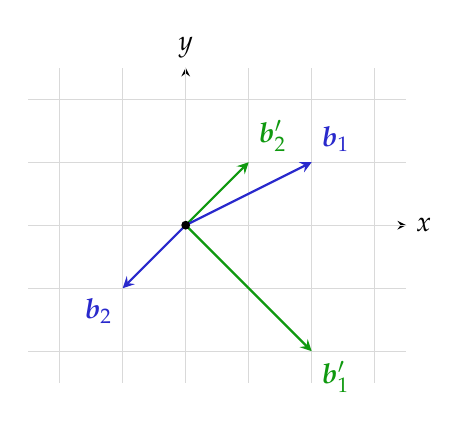
\begin{tikzpicture}[scale=0.8, >=stealth]

                            % Axes
                            \draw[->] (-2.5,0) -- (3.5,0) node[right] {$x$};
                            \draw[->] (0,-2.5) -- (0,2.5) node[above] {$y$};

                            % Grid
                            \draw[help lines, gray!30] (-2.5,-2.5) grid (3.5,2.5);

                            % New basis vectors b1', b2'
                            \draw[->, thick, white!10!green!60!black] (0,0) -- (2,-2) node[below right] {$\vect{b}'_1$};
                            \draw[->, thick, white!10!green!60!black] (0,0) -- (1,1) node[above right] {$\vect{b}'_2$};

                            % Original basis vectors b1, b2
                            \draw[->, thick, white!20!blue!80!black] (0,0) -- (2,1) node[above right] {$\vect{b}_1$};
                            \draw[->, thick, white!20!blue!80!black] (0,0) -- (-1,-1) node[below left] {$\vect{b}_2$};

                            % Origin
                            \fill (0,0) circle (2pt);

                        \end{tikzpicture}
                    }
                    \vspace{0.1em}

              \item[b.] Compute the matrix $\mat{P}_1$ that performs a basis change from $B'$ to $B$.

                    \vspace{1em}

                    Denote $\mat{S}_B$ and $\mat{S}_{B'}$ as the change-of-basis matrices from $B$ and $B'$ to $E_2$,
                    the standard basis of $\R^2$, respectively:
                    \[
                        \mat{S}_B =
                        \begin{bmatrix}
                            \begin{array}{@{\negthickspace}i{3}i{3}@{\;\;}}
                                2 & -1 \\
                                1 & -1 \\
                            \end{array}
                        \end{bmatrix}
                        \qquad
                        \mat{S}_{B'} =
                        \begin{bmatrix}
                            \begin{array}{@{\,}i{3}i{2}@{\;\;}}
                                2  & 1 \\
                                -2 & 1 \\
                            \end{array}
                        \end{bmatrix}
                    \]
                    Then
                    \[
                        \mat{P}_1 = \mat{S}_B^{-1} \mat{S}_{B'} =
                        \begin{bmatrix}
                            \begin{array}{@{\negthickspace}i{3}i{3}@{\;\;}}
                                1 & -1 \\
                                1 & -2 \\
                            \end{array}
                        \end{bmatrix}
                        \begin{bmatrix}
                            \begin{array}{@{\,}i{3}i{2}@{\;\;}}
                                2  & 1 \\
                                -2 & 1 \\
                            \end{array}
                        \end{bmatrix}
                        =
                        \begin{bmatrix}
                            \begin{array}{@{\!\!}i{3}i{3}@{\;\;}}
                                4 & 0  \\
                                6 & -1 \\
                            \end{array}
                        \end{bmatrix}
                    \]

              \item[c.] Let $C = (\vect{c}_1, \vect{c}_2, \vect{c}_3)$, where $\vect{c}_1, \vect{c}_2, \vect{c}_2$ are three
                    vectors of $\R^3$ defined in $E_3$, the standard basis of $\R^3$:
                    \[
                        \vect{c}_1 = \begin{bmatrix}
                            \begin{array}{@{\,}i{3}}
                                1 \\ 2 \\ -1
                            \end{array}
                        \end{bmatrix}
                        \quad
                        \vect{c}_2 = \begin{bmatrix}
                            \begin{array}{@{\,}i{3}}
                                0 \\ -1 \\ 2
                            \end{array}
                        \end{bmatrix}
                        \quad
                        \vect{c}_3 = \begin{bmatrix}
                            \begin{array}{@{\,}i{3}}
                                1 \\ 0 \\ -1
                            \end{array}
                        \end{bmatrix}
                    \]

                    \begin{enumerate}
                        \item[i.] Show that $C$ is a basis of $\R^3$ (for example, by using determinants).

                              \vspace{1em}

                              The matrix with columns $\vect{c}_1, \vect{c}_2, \vect{c}_3$ has full rank, so $C$
                              is a basis of $\R^3$:
                              \[
                                  \det \args{
                                      \begin{bmatrix}
                                          \begin{array}{@{}i{3}i{3}i{3}@{\;\;}}
                                              1  & 0  & 1  \\
                                              2  & -1 & 0  \\
                                              -1 & 2  & -1 \\
                                          \end{array}
                                      \end{bmatrix}
                                  }
                                  =
                                  \det \args{
                                      \begin{bmatrix}
                                          \begin{array}{@{}i{3}i{3}@{\;\;}}
                                              -1 & 0  \\
                                              2  & -1 \\
                                          \end{array}
                                      \end{bmatrix}
                                  }
                                  +
                                  \det \args{
                                      \begin{bmatrix}
                                          \begin{array}{@{}i{3}i{3}@{\;\;}}
                                              2  & -1 \\
                                              -1 & 2  \\
                                          \end{array}
                                      \end{bmatrix}
                                  }
                                  = 4
                              \]

                        \item[ii.] Let us call $C' = (\vect{c}'_1, \vect{c}'_2, \vect{c}'_3)$ the standard basis of
                              $\R^3$.  Determine the matrix $\mat{P}_2$ that performs the change of basis from $C$ to
                              $C'$.

                              \vspace{1em}
                              $\mat{P}_2$ is exactly the matrix above, with columns $\vect{c}_1, \vect{c}_2, \vect{c}_3$:
                              \[
                                  \mat{P}_2 =
                                  \begin{bmatrix}
                                      \begin{array}{@{}i{3}i{3}i{3}@{\;\;}}
                                          1  & 0  & 1  \\
                                          2  & -1 & 0  \\
                                          -1 & 2  & -1 \\
                                      \end{array}
                                  \end{bmatrix}
                              \]
                    \end{enumerate}

              \item[d.] We consider a homomorphism $\Phi : \R^2 \rightarrow \R^3$, such that
                    \[
                        \begin{aligned}
                            \Phi(\vect{b}_1 + \vect{b}_2) & = \vect{c}_2 + \vect{c}_3                  \\
                            \Phi(\vect{b}_1 - \vect{b}_2) & = 2 \vect{c}_1 - \vect{c}_2 + 3 \vect{c}_3 \\
                        \end{aligned}
                    \]
                    where $B = (\vect{b}_1, \vect{b}_2)$ and $C = (\vect{c}_1, \vect{c}_2, \vect{c}_3)$
                    are ordered bases of $\R^2$ and $\R^3$, respectively.

                    Determine the transformation matrix $\mat{A}_\Phi$ of $\Phi$ with respect to the ordered
                    bases $B$ and $C$.

                    \vspace{0.5em}
                    Reformulating, we have
                    \[
                        \mat{A}_\Phi
                        \begin{bmatrix}
                            \begin{array}{@{\;}c@{\;}}
                                1 \\ 1
                            \end{array}
                        \end{bmatrix}_{\!B}
                        = \begin{bmatrix}
                            \begin{array}{@{\;}c@{\;}}
                                0 \\ 1 \\ 1
                            \end{array}
                        \end{bmatrix}_{\!C}
                        \quad
                        \text{and}
                        \quad
                        \mat{A}_\Phi
                        \begin{bmatrix}
                            \begin{array}{@{\,}i{3}@{\;}}
                                1 \\ -1
                            \end{array}
                        \end{bmatrix}_{\!B}
                        = \begin{bmatrix}
                            \begin{array}{@{\,}i{3}@{\;}}
                                2 \\ -1 \\ 3
                            \end{array}
                        \end{bmatrix}_{\!C}
                    \]
                    which we combine and solve:
                    \[
                        \begin{aligned}
                            \mat{A}_\Phi
                            \begin{bmatrix}
                                \begin{array}{@{}i{2}i{3}@{\;\,}}
                                    1 & 1  \\
                                    1 & -1 \\
                                \end{array}
                            \end{bmatrix}
                             & = \begin{bmatrix}
                                     \begin{array}{@{}i{3}i{3}@{\;\,}}
                                    0 & 2  \\
                                    1 & -1 \\
                                    1 & 3  \\
                                \end{array}
                                 \end{bmatrix}
                            \\
                            \iff \quad
                            \mat{A}_\Phi
                             & =
                            \begin{bmatrix}
                                \begin{array}{@{}i{3}i{3}@{\;\,}}
                                    0 & 2  \\
                                    1 & -1 \\
                                    1 & 3  \\
                                \end{array}
                            \end{bmatrix}
                            \begin{bmatrix}
                                \begin{array}{@{}i{2}i{3}@{\;\,}}
                                    1 & 1  \\
                                    1 & -1 \\
                                \end{array}
                            \end{bmatrix}
                            ^{-1}
                            \\
                             & =
                            \begin{bmatrix}
                                \begin{array}{@{}i{3}i{3}@{\;\,}}
                                    0 & 2  \\
                                    1 & -1 \\
                                    1 & 3  \\
                                \end{array}
                            \end{bmatrix}
                            \begin{bmatrix}
                                \begin{array}{cc}
                                    \sfrac{1}{2} & \;\;\;\sfrac{1}{2} \\
                                    \sfrac{1}{2} & \sfrac{-1}{2}      \\
                                \end{array}
                            \end{bmatrix}
                            \\
                             & =
                            \begin{bmatrix}
                                \begin{array}{@{}i{3}i{3}@{\;\,}}
                                    1 & -1 \\
                                    0 & 1  \\
                                    2 & -1 \\
                                \end{array}
                            \end{bmatrix}
                        \end{aligned}
                    \]

              \item[e.] Determine $\mat{A}'_\Phi$, the transformation matrix with respect to the bases $B'$ and $C'$.

                    \vspace{1em}

                    We already computed $\mat{P}_1$, the change of basis matrix from $B'$ to $B$, and $\mat{P}_2$, the
                    change of basis matrix from $C$ to $C'$, so composing these with $\mat{A}_\Phi$ we have
                    \[
                        \mat{A}'_\Phi = \mat{P}_2 \mat{A}_\Phi \mat{P}_1
                    \]
                    Spelling this out,
                    \[
                        \underbrace{
                            [\vect{x}]_{B'}
                        }_{\text{coords in } B'}
                        \xrightarrow{\quad \text{\small $\mat{P}_1$} \quad}
                        \underbrace{
                            [\vect{x}]_B
                        }_{\text{coords in } B}
                        \xrightarrow{\quad \text{\small $\mat{A}_\Phi$} \quad}
                        \underbrace{
                            [\Phi(\vect{x})]_C
                        }_{\text{coords in } C}
                        \xrightarrow{\quad \text{\small $\mat{P}_2$} \quad}
                        \underbrace{
                            [\Phi(\vect{x})]_{C'}
                        }_{\text{coords in } C'}
                    \]

                    We compute $\mat{A}'_\Phi$:
                    \[
                        \mat{A}'_\Phi =
                        \begin{bmatrix}
                            \begin{array}{@{}i{3}i{3}i{3}@{\;\;}}
                                1  & 0  & 1  \\
                                2  & -1 & 0  \\
                                -1 & 2  & -1 \\
                            \end{array}
                        \end{bmatrix}
                        \begin{bmatrix}
                            \begin{array}{@{}i{3}i{3}@{\;\,}}
                                1 & -1 \\
                                0 & 1  \\
                                2 & -1 \\
                            \end{array}
                        \end{bmatrix}
                        \begin{bmatrix}
                            \begin{array}{@{\!\!}i{3}i{3}@{\;\;}}
                                4 & 0  \\
                                6 & -1 \\
                            \end{array}
                        \end{bmatrix}
                        =
                        \begin{bmatrix}
                            \begin{array}{@{\!}i{4}i{3}@{\;\,}}
                                0   & 2  \\
                                -10 & 3  \\
                                12  & -4 \\
                            \end{array}
                        \end{bmatrix}
                    \]

              \item[f.] Let us consider the vector $\vect{x} \in \R^2$, whose coordinates in $B'$ are
                    $
                        \begin{bmatrix}
                            \begin{array}{@{\;}c@{\;}}
                                2 \\ 3
                            \end{array}
                        \end{bmatrix}
                    $.

                    In other words, $\vect{x} = 2 \vect{b}'_1 + 3 \vect{b}'_2$.

                    \begin{enumerate}
                        \item[i.] Calculate the coordinates of $\vect{x}$ in $B$.
                              \[
                                  [\vect{x}]_B = \mat{P}_1 [\vect{x}]_{B'} =
                                  \begin{bmatrix}
                                      \begin{array}{@{\!\!}i{3}i{3}@{\;\;}}
                                          4 & 0  \\
                                          6 & -1 \\
                                      \end{array}
                                  \end{bmatrix}
                                  \begin{bmatrix}
                                      \begin{array}{@{\;}c@{\;}}
                                          2 \\ 3
                                      \end{array}
                                  \end{bmatrix}
                                  =
                                  \begin{bmatrix}
                                      \begin{array}{@{\;}c@{\;}}
                                          8 \\ 9
                                      \end{array}
                                  \end{bmatrix}
                              \]

                        \item[ii.] Based on that, compute the coordinates of $\Phi(\vect{x})$ expressed in $C$.
                              \[
                                  [\Phi(\vect{x})]_C =
                                  \mat{A}_\Phi [\vect{x}]_B =
                                  \begin{bmatrix}
                                      \begin{array}{@{}i{3}i{3}@{\;\,}}
                                          1 & -1 \\
                                          0 & 1  \\
                                          2 & -1 \\
                                      \end{array}
                                  \end{bmatrix}
                                  \begin{bmatrix}
                                      \begin{array}{@{\;}c@{\;}}
                                          8 \\ 9
                                      \end{array}
                                  \end{bmatrix}
                                  =
                                  \begin{bmatrix}
                                      \begin{array}{@{}i{3}@{\;}}
                                          -1 \\ 9 \\ 7
                                      \end{array}
                                  \end{bmatrix}
                              \]

                        \item[iii.] Then write $\Phi(\vect{x})$ in terms of $\vect{c}'_1, \vect{c}'_2, \vect{c}'_3$.
                              \[
                                  [\Phi(\vect{x})]_{C'} =
                                  \mat{P}_2 [\Phi(\vect{x})]_C =
                                  \begin{bmatrix}
                                      \begin{array}{@{}i{3}i{3}i{3}@{\;\;}}
                                          1  & 0  & 1  \\
                                          2  & -1 & 0  \\
                                          -1 & 2  & -1 \\
                                      \end{array}
                                  \end{bmatrix}
                                  \begin{bmatrix}
                                      \begin{array}{@{}i{3}@{\;}}
                                          -1 \\ 9 \\ 7
                                      \end{array}
                                  \end{bmatrix}
                                  =
                                  \begin{bmatrix}
                                      \begin{array}{@{}i{4}@{\;}}
                                          6 \\ -11 \\ 12
                                      \end{array}
                                  \end{bmatrix}
                              \]

                        \item[iv.] Use the representation of $\vect{x}$ in $B'$ and the matrix $\mat{A}'_\Phi$ to find this result directly.
                              \[
                                  [\Phi(\vect{x})]_{C'} =
                                  \mat{A}'_\Phi [\vect{x}]_{B'} =
                                  \begin{bmatrix}
                                      \begin{array}{@{\!}i{4}i{3}@{\;\,}}
                                          0   & 2  \\
                                          -10 & 3  \\
                                          12  & -4 \\
                                      \end{array}
                                  \end{bmatrix}
                                  \begin{bmatrix}
                                      \begin{array}{@{\;}c@{\;}}
                                          2 \\ 3
                                      \end{array}
                                  \end{bmatrix}
                                  =
                                  \begin{bmatrix}
                                      \begin{array}{@{}i{4}@{\;}}
                                          6 \\ -11 \\ 12
                                      \end{array}
                                  \end{bmatrix}
                              \]

                    \end{enumerate}

                    \begin{figure}
                        \centering
                        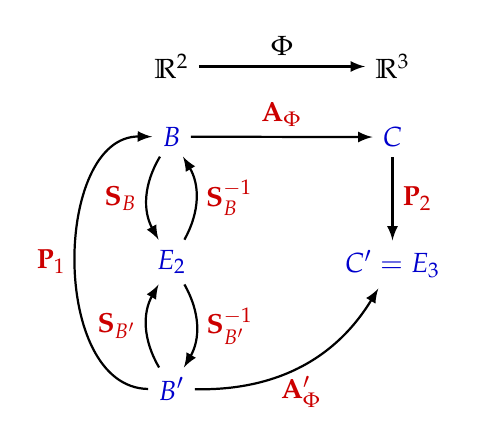
\begin{tikzpicture}[
                                ->,
                                >=latex,
                                thick,
                                node distance=4em and 6em
                            ]
                            \tikzset{
                                labelblue/.style = {text=blue!80!black},
                                labelred/.style = {text=red!80!black}
                            }

                            % Vector spaces
                            \node (R2) {$\R^2$};
                            \node[right=of R2] (R3) {$\R^3$};
                            \draw[->] (R2) -- node[above] {$\Phi$} (R3);

                            % Left column (B, E_2, B')
                            \node[below=1em of R2, labelblue] (B) {$B$};
                            \node[below=3em of B, labelblue] (E2) {$E_2$};
                            \node[below=3em of E2, labelblue] (Bp) {$B'$};

                            \path (Bp) edge [bend left] node [left, labelred] {$\mat{S}_{B'}$} (E2);
                            \path (E2) edge [bend left] node [right, labelred] {$\mat{S}_{B'}^{-1}$} (Bp);
                            \path (B) edge [bend right] node [left, labelred] {$\mat{S}_B$} (E2);
                            \path (E2) edge [bend right] node [right, labelred] {$\mat{S}_B^{-1}$} (B);
                            \path (Bp) edge [bend left=90] node [left, labelred] {$\mat{P}_1$} (B);

                            % Right column (C, E_3, C')
                            \node[below=1em of R3, labelblue] (C) {$C$};
                            \node[below=3em of C, labelblue] (Cp) {$C' = E_3$};

                            \draw[->] (C) -- node[right, labelred] {$\mat{P}_2$} (Cp);

                            % Transformations (rightward arrows)
                            \draw[->] (B) -- node[above, labelred] {$\mat{A}_\Phi$} (C);
                            \path (Bp) edge [bend right] node [below, labelred] {$\mat{A}'_\Phi$} (Cp);

                        \end{tikzpicture}
                        \caption{Bases and matrices in Exercise 2.20}
                    \end{figure}

          \end{enumerate}

\end{enumerate}

\pagebreak

\section{Analytic geometry}

\begin{enumerate}

    \item[3.1] Show that $\inner{\cdot}{\cdot}$ defined for all $\x = [x_1, x_2]^\top \in \R^2$ and
          $\y = [y_1, y_2]^\top \in \R^2$ by
          \[
              \inner{\x}{\y} = x_1 y_1 - (x_1 y_2 + x_2 y_1) + 2 x_2 y_2
          \]
          is an inner product.

          \vspace{1em}

          An inner product must be:

          \subsubsubsection{Symmetric}
          \[
              \forall \x, \y \in \R^2 : \inner{\x}{\y} = \inner{\y}{\x}
          \]

          \subsubsubsection{Bilinear}
          \[
              \forall \x, \y, \z \in \R^2, \;
              \forall \lambda, \phi \in \R :
              \begin{cases}
                  \inner{ \lambda \x + \phi \y }{ \z } = \lambda \inner{\x}{\z} + \phi \inner{\y}{\z}, \\
                  \inner{ \x }{ \lambda \y + \phi \z } = \lambda \inner{\x}{\y} + \phi \inner{\x}{\z}. \\
              \end{cases}
          \]

          \subsubsubsection{Positive definite}
          \[
              \forall \x \in \R^2 \setminus \set{\vect{0}} :
              \inner{\x}{\x} > 0,
              \qquad
              \inner{\vect{0}}{\vect{0}} = 0
          \]

          That the given $\inner{\cdot}{\cdot}$ is symmetric is obvious.  For bilinearity, consider that fixing
          one argument while holding the other constant, there are only linear terms in the components of each (no
          quadratic terms).  For positive definiteness, consider
          \[
              \begin{aligned}
                  \inner{\x}{\x} & = x_1^2 - 2 x_1 x_2 + 2 x_2^2 \\
                                 & = (x_1 - x_2)^2 + x_2^2
              \end{aligned}
          \]
          which is always positive for non-zero $x_1, x_2$, and $\inner{\vect{0}}{\vect{0}} = 0$, as required.

          This inner product may be represented with the following symmetric positive definite matrix:
          \[
              \begin{aligned}
                  \mat{A} :=
                  \begin{bmatrix}
                      \begin{array}{@{}i{3}i{3}@{\;\;}}
                          1  & -1 \\
                          -1 & 2  \\
                      \end{array}
                  \end{bmatrix}
                  \qquad
                  \inner{\x}{\y} = \x^\top \mat{A} \y
              \end{aligned}
          \]

          \pagebreak

    \item[3.2] Consider $\R^2$ with $\inner{\cdot}{\cdot}$ defined for all $\x, \y$ in $\R^2$ as
          \[
              \inner{\x}{\y} = \x^\top
              \underbrace{
                  \begin{bmatrix}
                      2 & 0 \\
                      1 & 2 \\
                  \end{bmatrix}
              }_{
              \mat{A} :=
              }
              \y
          \]
          Is $\inner{\cdot}{\cdot}$ an inner product?

          \vspace{1em}

          No.  An inner product may only be defined by a symmetric positive definite matrix.  Since $\mat{A}$ is
          not symmetric, $\inner{\cdot}{\cdot}$ is not symmetric in its arguments.

    \item[3.3] Compute the distance between
          \[
              \x = \begin{bmatrix}
                  \begin{array}{i{1}}
                      1 \\ 2 \\ 3
                  \end{array}
              \end{bmatrix}
              \qquad
              \y = \begin{bmatrix}
                  \begin{array}{@{}i{3}@{\,}}
                      -1 \\ -1 \\ 0
                  \end{array}
              \end{bmatrix}
          \]

          \begin{enumerate}
              \item[a.] Using $\inner{\x}{\y} = \x^\top \y$
                    \[
                        \x - \y = \begin{bmatrix}
                            \begin{array}{i{1}}
                                2 \\ 3 \\ 3
                            \end{array}
                        \end{bmatrix}
                        \qquad
                        \begin{aligned}
                            d(\x, \y) & = \norm{ \x - \y }                    \\
                                      & = \sqrt{\inner{ \x - \y }{ \x - \y }} \\
                                      & = \sqrt{22}                           \\
                                      & \approx 4.69
                        \end{aligned}
                    \]

              \item[b.] Using $\inner{\x}{\y} = \x^\top \mat{A} \y, \quad \mat{A} :=
                        \begin{bmatrix}
                            \begin{array}{@{\;}i{1}i{3}i{3}@{\;}}
                                2 & 1  & 0  \\
                                1 & 3  & -1 \\
                                0 & -1 & 2  \\
                            \end{array}
                        \end{bmatrix}
                    $
                    \[
                        \mat{A} (\vect{x} - \vect{y}) =
                        \begin{bmatrix}
                            \begin{array}{i{1}}
                                7 \\ 8 \\ 3
                            \end{array}
                        \end{bmatrix}
                        \qquad
                        (\vect{x} - \vect{y})^\top \mat{A} (\vect{x} - \vect{y}) = 47
                        \qquad
                        d(\x, \y) = \sqrt{47} \approx 6.86
                    \]

          \end{enumerate}

    \item[3.4] Compute the angle between
          \[
              \x = \begin{bmatrix}
                  \begin{array}{@{\;}i{1}@{\;}}
                      1 \\ 2
                  \end{array}
              \end{bmatrix}
              \qquad
              \y = \begin{bmatrix}
                  \begin{array}{@{}i{3}@{\,}}
                      -1 \\ -1
                  \end{array}
              \end{bmatrix}
          \]

          \begin{enumerate}
              \item[a.] Using $\inner{\x}{\y} = \x^\top \y$
                    \[
                        \cos \theta
                        = \frac{ \inner{\x}{\y} }{ \norm{\x} \norm{\y} }
                        \qquad
                        \inner{\x}{\y} = -3
                        \qquad
                        \norm{\x} = \sqrt{5}
                        \qquad
                        \norm{\y} = \sqrt{2}
                        \qquad
                        \theta \approx 161.6\degree
                    \]

              \item[b.] Using $\inner{\x}{\y} = \x^\top \mat{B} \y, \quad \mat{B} :=
                        \begin{bmatrix}
                            \begin{array}{@{\;}i{1}i{1}@{\;}}
                                2 & 1 \\
                                1 & 3 \\
                            \end{array}
                        \end{bmatrix}
                    $
                    \[
                        \mat{B} \x =
                        \begin{bmatrix}
                            \begin{array}{@{\,}i{1}@{\,}}
                                4 \\ 7
                            \end{array}
                        \end{bmatrix}
                        \quad
                        \mat{B} \y =
                        \begin{bmatrix}
                            \begin{array}{@{}i{3}@{\,}}
                                -3 \\ -4
                            \end{array}
                        \end{bmatrix}
                        \quad \;\;
                        \inner{\x}{\y} = -11
                        \quad \;\;
                        \norm{\x} = \sqrt{18}
                        \quad \;\;
                        \norm{\y} = \sqrt{7}
                        \quad \;\;
                        \theta \approx 168.5\degree
                    \]
          \end{enumerate}

    \item[3.5] Consider the Euclidean vector space $\R^5$ with the dot product. A subspace $U \subseteq \R^5$ and
          $\x \in \R^5$ are given by
          \[
              U = \Span \args{
                  \begin{bmatrix}
                      \begin{array}{@{}i{3}@{\;}}
                          0 \\ -1 \\ 2 \\ 0 \\ 2
                      \end{array}
                  \end{bmatrix}
                  \! ,
                  \begin{bmatrix}
                      \begin{array}{@{}i{3}@{\;}}
                          1 \\ -3 \\ 1 \\ -1 \\ 2
                      \end{array}
                  \end{bmatrix}
                  \! ,
                  \begin{bmatrix}
                      \begin{array}{@{}i{3}@{\;}}
                          -3 \\ 4 \\ 1 \\ 2 \\ 1
                      \end{array}
                  \end{bmatrix}
                  \! ,
                  \begin{bmatrix}
                      \begin{array}{@{}i{3}@{\;}}
                          -1 \\ -3 \\ 5 \\ 0 \\ 7
                      \end{array}
                  \end{bmatrix}
              }
              \qquad
              \x =
              \begin{bmatrix}
                  \begin{array}{@{}i{3}@{\;}}
                      -1 \\ -9 \\ -1 \\ 4 \\ 1
                  \end{array}
              \end{bmatrix}
          \]

          \begin{enumerate}
              \item[a.] Determine the orthogonal projection $\pi_U(\x)$ of $\x$ onto $U$.
              \item[b.] Determine the distance $d(\x, U)$.

                    \vspace{1em}

                    Let $\mat{B} = [ \vect{b}_1 \; \vect{b}_2 \; \vect{b}_3 \; \vect{b}_4  ]$, where the respective
                    $\vect{b}_i$ are the vectors in the span of $U$ as above, and let $\bm{\lambda} = [ \lambda_1 \;
                        \lambda_2 \; \lambda_3 \; \lambda_4 ]^\top$, such that $\pi_U(\x) = \mat{B}\bm{\lambda}$, where
                    $\bm{\lambda}$ gives the coordinates of the projection of $\x$ onto $U$, relative to the ordered
                    basis of $U$.

                    The residual, $\x - \mat{B} \bm{\lambda}$, must be orthogonal to each basis vector:
                    \[
                        \begin{array}{c}
                            \inner{\vect{b}_1}{\x - \mat{B}\bm{\lambda}} = 0 \\ \vdots \\ [2pt]
                            \inner{\vect{b}_4}{\x - \mat{B}\bm{\lambda}} = 0 \\
                        \end{array}
                    \]
                    which, given bilinearity and our use of the standard dot product, is equivalently:
                    \[
                        \begin{array}{c}
                            \inner{\vect{b}_1}{\mat{B}\bm{\lambda}} = \inner{\vect{b}_1}{\x} \\ \vdots \\ [2pt]
                            \inner{\vect{b}_4}{\mat{B}\bm{\lambda}} = \inner{\vect{b}_4}{\x} \\
                        \end{array}
                        \quad
                        \iff
                        \quad
                        \begin{array}{c}
                            \vect{b}_1^\top \mat{B}\bm{\lambda}= \vect{b}_1^\top \x \\ \vdots \\ [2pt]
                            \vect{b}_4^\top \mat{B}\bm{\lambda}= \vect{b}_4^\top \x \\
                        \end{array}
                        \quad
                        \iff
                        \quad
                        \mat{B}^\top \mat{B} \bm{\lambda} = \mat{B}^\top \x \\ [2pt]
                    \]

                    Note, we find $\mat{B}$ is rank 3 — its columns are linearly dependent.  Consequently, its Gram
                    matrix ($\mat{B}^\top \mat{B}$) is singular.  Below, we proceed to find $\bm{\lambda}'$ with
                    Gaussian elimination, but note it may instead be computed directly by inverting the Gram matrix in
                    the expression on the right above — though only if the Gram matrix is invertible.

                    So, discarding $\vect{b}_4$ and $\lambda_4$, let $\mat{B}' = [\vect{b}_1  \; \vect{b}_2 \;
                        \vect{b}_3]$, eliminate $[ \, \mat{B}'^\top \mat{B} \, \mid \, \mat{B}'^\top \x \, ]
                        \rightsquigarrow [ \; \mat{I} \, \mid \, \bm{\lambda}' \; ]$, and finally find $\pi_U(\x) = \mat{B}
                        \bm{\lambda}'$, and the corresponding residual:
                    \[
                        \begin{aligned}
                            \begin{bmatrix}
                                \begin{array}{@{}i{3}i{4}i{4}|i{4}@{\;}}
                                    9 & 9   & 0   & 9   \\
                                    9 & 16  & -14 & 23  \\
                                    0 & -14 & 31  & -25 \\
                                \end{array}
                            \end{bmatrix}
                             & \rightsquigarrow
                            \begin{bmatrix}
                                \begin{array}{@{}i{2}i{4}i{4}|i{4}@{\;}}
                                    1 & 1   & 0   & 1   \\
                                    0 & 7   & -14 & 14  \\
                                    0 & -14 & 31  & -25 \\
                                \end{array}
                            \end{bmatrix}
                            \\
                             & \rightsquigarrow
                            \begin{bmatrix}
                                \begin{array}{@{}i{2}i{4}i{4}|i{4}@{\;}}
                                    1 & 1 & 0  & 1 \\
                                    0 & 1 & -2 & 2 \\
                                    0 & 0 & 3  & 3 \\
                                \end{array}
                            \end{bmatrix}
                            \\
                             & \rightsquigarrow
                            \begin{bmatrix}
                                \begin{array}{@{}i{2}i{4}i{4}|i{4}@{\;}}
                                    1 & 0 & 0 & -3 \\
                                    0 & 1 & 0 & 4  \\
                                    0 & 0 & 1 & 1  \\
                                \end{array}
                            \end{bmatrix}
                        \end{aligned}
                        \qquad
                        \begin{aligned}
                            \pi_U(\x)      & =
                            \begin{bmatrix}
                                \begin{array}{@{}i{3}@{\;}}
                                    1 \\ -5  \\ -1  \\ -2 \\ 3
                                \end{array}
                            \end{bmatrix}
                            \\
                            \x - \pi_U(\x) & =
                            \begin{bmatrix}
                                \begin{array}{@{}i{3}@{\;}}
                                    -2 \\ -4  \\ 0 \\ 6 \\ -2
                                \end{array}
                            \end{bmatrix}
                        \end{aligned}
                    \]
                    Compute the distance, $d(\x, U) = \norm{\x - \pi_U(\x)} = \sqrt{60} = 2 \sqrt{15} \approx 7.75$.

                    \pagebreak
          \end{enumerate}

    \item[3.6] Consider $\R^3$ with the inner product $\inner{\x}{\y} := \x^\top \mat{A} \y$, where
          \[
              \mat{A} :=
              \begin{bmatrix}
                  \begin{array}{@{}i{2}i{3}i{3}@{\;}}
                      2 & 1  & 0  \\
                      1 & 2  & -1 \\
                      0 & -1 & 2  \\
                  \end{array}
              \end{bmatrix}
          \]
          Furthermore, define $\vect{e}_1, \vect{e}_2, \vect{e}_3$ to be the standard / canonical basis in
          $\R^3$.

          \begin{enumerate}
              \item[a.] Determine the orthogonal projection $\pi_U(\vect{e}_2)$ of $\vect{e}_2$ onto
                    \[
                        U = \Span \args{\vect{e}_1, \vect{e}_3}.
                    \]

              \item[b.] Compute the distance $d(\vect{e}_2, U)$.

              \item[c.] Draw the scenario, standard basis vectors and $\pi_U(\vect{e}_2)$.
          \end{enumerate}

          \vspace{1em}

          Let $\mat{B} = [\vect{e}_1 \; \vect{e}_3]$, and let $\bm{\lambda} = [\lambda_1 \; \lambda_2]^\top$
          be the coordinates of $\pi_U(\vect{e}_2)$ in the ordered basis of $U$, such that
          $\pi_U(\vect{e}_2) = \mat{B} \bm{\lambda}$.  Then
          \[
              \begin{aligned}
                  \inner{ \vect{e}_1 }{ \vect{e}_2 - \mat{B} \bm{\lambda} } = 0 \\
                  \inner{ \vect{e}_3 }{ \vect{e}_2 - \mat{B} \bm{\lambda} } = 0 \\
              \end{aligned}
              \quad
              \iff
              \quad
              \begin{aligned}
                  \vect{e}_1^\top \mat{A} \vect{e}_2 = \vect{e}_1^\top \mat{A} \mat{B} \bm{\lambda} \\
                  \vect{e}_3^\top \mat{A} \vect{e}_2 = \vect{e}_3^\top \mat{A} \mat{B} \bm{\lambda} \\
              \end{aligned}
              \quad
              \iff
              \quad
              \mat{B}^\top \mat{A} \vect{e}_2 = \mat{B}^\top \mat{A} \mat{B} \bm{\lambda}
          \]
          Computing
          \[
              \mat{B}^\top \mat{A} \vect{e}_2 =
              \mat{B}^\top \!
              \begin{bmatrix}
                  \begin{array}{@{}i{3}@{\;}}
                      1 \\ 2 \\ -1
                  \end{array}
              \end{bmatrix}
              =
              \begin{bmatrix}
                  \begin{array}{@{}i{3}@{\;}}
                      1 \\ -1
                  \end{array}
              \end{bmatrix}
              \qquad
              \mat{B}^\top \mat{A} \mat{B} =
              \mat{B}^\top
              \begin{bmatrix}
                  \begin{array}{@{}i{2}i{3}@{\;}}
                      2 & 0  \\
                      1 & -1 \\
                      0 & 2  \\
                  \end{array}
              \end{bmatrix}
              =
              \begin{bmatrix}
                  \begin{array}{@{\;}i{1}i{1}@{\;}}
                      2 & 0 \\
                      0 & 2 \\
                  \end{array}
              \end{bmatrix}
          \]
          \[
              \bm{\lambda} =
              \begin{bmatrix}
                  \begin{array}{@{\,}r}
                      \sfrac{1}{2} \\ -\sfrac{1}{2}
                  \end{array}
              \end{bmatrix}
              \qquad
              \pi_U(\vect{e}_2) =
              \begin{bmatrix}
                  \begin{array}{@{\,}r}
                      \sfrac{1}{2} \\ 0 \\ -\sfrac{1}{2}
                  \end{array}
              \end{bmatrix}
              \qquad
              \vect{e}_2 - \pi_U(\vect{e}_2) =
              \begin{bmatrix}
                  \begin{array}{@{\,}r}
                      -\sfrac{1}{2} \\ 1 \\ \sfrac{1}{2}
                  \end{array}
              \end{bmatrix}
          \]
          Finally,
          \[
              \begin{aligned}
                  d(\vect{e}_2, U) & = \norm{ \vect{e}_2 - \pi_U(\vect{e}_2) }                                                   \\
                                   & = \sqrt{( \vect{e}_2 - \pi_U(\vect{e}_2) )^\top \mat{A} ( \vect{e}_2 - \pi_U(\vect{e}_2) )} \\
                                   & = \sqrt{
                      \begin{bmatrix}
                          \begin{array}{@{\,}r}
                              -\sfrac{1}{2} \\ 1 \\ \sfrac{1}{2}
                          \end{array}
                      \end{bmatrix}^\top
                      \begin{bmatrix}
                          \begin{array}{c}
                              0 \\ 1 \\ 0
                          \end{array}
                      \end{bmatrix}
                  }
                  \\
                                   & = 1.
              \end{aligned}
          \]

          \vspace{1em}
          \makebox[\linewidth][c]{%
              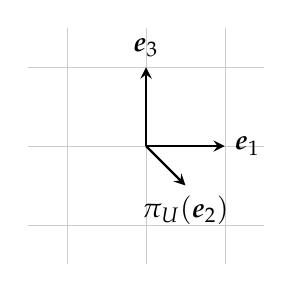
\begin{tikzpicture}[>=stealth]
                  % Grid
                  \draw[help lines, gray!40] (-1.5, -1.5) grid (1.5, 1.5);

                  % U basis
                  \draw[->, thick, black] (0, 0) -- (1, 0) node[right] {$\vect{e}_1$};
                  \draw[->, thick, black] (0, 0) -- (0, 1) node[above] {$\vect{e}_3$};

                  % Projection
                  \draw[->, thick, black] (0, 0) -- (0.5, -0.5) node[below] {$\pi_U(\vect{e}_2)$};
              \end{tikzpicture}
          }

          \pagebreak

    \item[3.7] Let $V$ be a vector space and $\pi$ an endomorphism of $V$.

          \begin{enumerate}
              \item[a.] Prove that $\pi$ is a projection if and only if $\id_V - \pi$ is a projection, where $\id_V$
                    is the identity endomorphism on $V$.

                    \begin{proof}
                        Define $\rho = \id_V - \pi$.  Then
                        \[
                            \rho^2 = \id_V - 2 \pi + \pi^2.
                        \]
                        \[
                            \rho^2 = \rho
                            \begin{aligned}
                                 & \quad \iff \quad
                                \id_V - 2 \pi + \pi^2 = \id_V - \pi \\
                                 & \quad \iff \quad
                                \pi^2 = \pi                         \\
                            \end{aligned}
                        \]
                    \end{proof}

              \item[b.] Assume now that $\pi$ is a projection.  Calculate $\Img(\id_V - \pi)$ and $\ker(\id_V
                        - \pi)$ as a function of $\Img(\pi)$ and $\ker(\pi)$.
                    \[
                        \Img(\id_V - \pi) = \ker(\pi)
                    \]
                    \begin{proof}
                        Let $\vect{v} \in \Img(\id_V - \pi)$, let $\vect{u} \in V$ be a preimage of $\vect{v}$ under $\id_V - \pi$, and consider:
                        \[
                            \begin{aligned}
                                \vect{v}      & = (\id_V - \pi)(\vect{u})                   \\
                                              & = \vect{u} - \pi(\vect{u}),                 \\
                                \pi(\vect{v}) & = \pi(\vect{u}) - \pi(\pi(\vect{u}))        \\
                                              & = \pi(\vect{u}) - \pi(\vect{u})             \\
                                              & = \vect{0} \implies \vect{v} \in \ker(\pi).
                            \end{aligned}
                        \]
                        Then let $\vect{w} \in \ker(\pi)$, and consider:
                        \[
                            \begin{aligned}
                                \pi(\vect{w})           & = \vect{0},                                         \\
                                (\id_V - \pi)(\vect{w}) & = \vect{w} - \pi(\vect{w})                          \\
                                                        & = \vect{w} \implies \vect{w} \in \Img(\id_V - \pi).
                            \end{aligned}
                        \]
                    \end{proof}

                    \[
                        \ker(\id_V - \pi) = \Img(\pi)
                    \]
                    \begin{proof}
                        Let $\vect{w} \in \ker(\id_V - \pi)$, and consider:
                        \[
                            \begin{alignedat}{2}
                                         &  & (\id_V - \pi)(\vect{w}) & = \vect{w} - \pi(\vect{w}) = \vect{0} \\
                                \iff     &  & \pi(\vect{w})           & = \vect{w}                            \\
                                \implies &  & \vect{w} \in \Img(\pi)  & .
                            \end{alignedat}
                        \]
                        Then let $\vect{v} \in \Img(\pi)$, let $\vect{u} \in V$ be a preimage of $\vect{v}$ under $\id_V - \pi$, and consider:
                        \[
                            \begin{aligned}
                                \pi(\vect{u})           & = \vect{v},                                         \\
                                (\id_V - \pi)(\vect{v}) & = \vect{v} - \pi(\vect{v})                          \\
                                                        & = \pi(\vect{u}) - \pi(\pi(\vect{u}))                \\
                                                        & = \pi(\vect{u}) - \pi(\vect{u})                     \\
                                                        & = \vect{0} \implies \vect{v} \in \ker(\id_V - \pi).
                            \end{aligned}
                        \]
                    \end{proof}
          \end{enumerate}

    \item[3.8] Using the Gram-Schmidt method, turn the basis $B = (\vect{b}_1, \vect{b}_2)$ of a two-dimensional
          subspace $U \subseteq \R^3$ into an orthonormal basis, $C = (\vect{c}_1, \vect{c}_2)$ of $U$, where
          \[
              \vect{b}_1 :=
              \begin{bmatrix}
                  \begin{array}{@{\;}i{1}@{\;}}
                      1 \\ 1 \\ 1
                  \end{array}
              \end{bmatrix} \! ,
              \qquad
              \vect{b}_2 :=
              \begin{bmatrix}
                  \begin{array}{@{}i{3}@{\;}}
                      -1 \\ 2 \\ 0
                  \end{array}
              \end{bmatrix} \! .
          \]
          Let $\vect{u}_1 = \vect{b}_1$.  Then let $\vect{u}_2 = \vect{b}_2 - \pi_{\vect{u}_1}\!(\vect{b}_2)$, where
          $\pi_{\vect{u}_1}$ is the projection operator onto the one-dimensional subspace spanned by $\vect{u}_1$.
          Assuming the standard dot product,
          \[
              \pi_{\vect{u}_1}(\vect{b}_2)
              = \frac{ \vect{u}_1 \vect{u}_1^\top }{ \norm{\vect{u}_1}^2 } \vect{b}_2
              = \frac{1}{3}
              \begin{bmatrix}
                  \begin{array}{@{\;}i{1}i{1}i{1}@{\;}}
                      1 & 1 & 1 \\
                      1 & 1 & 1 \\
                      1 & 1 & 1 \\
                  \end{array}
              \end{bmatrix}
              \begin{bmatrix}
                  \begin{array}{@{}i{3}@{\;}}
                      -1 \\ 2 \\ 0
                  \end{array}
              \end{bmatrix}
              =
              \frac{1}{3} \!
              \begin{bmatrix}
                  \begin{array}{@{\;}i{1}@{\;}}
                      1 \\ 1 \\ 1
                  \end{array}
              \end{bmatrix} \! ,
              \qquad
              \vect{u}_2 =
              \frac{1}{3} \!
              \begin{bmatrix}
                  \begin{array}{@{}i{3}@{\;}}
                      -4 \\ 5  \\ -1
                  \end{array}
              \end{bmatrix} \! .
          \]
          Normalizing each of $\vect{u}_1$ and $\vect{u}_2$, we define our orthonormal basis vectors to be:
          \[
              \vect{c}_1
              := \frac{ \vect{u}_1 }{ \norm {\vect{u}_1} }
              = \frac{\sqrt{3}}{3} \!
              \begin{bmatrix}
                  \begin{array}{@{\;}i{1}@{\;}}
                      1 \\ 1 \\ 1
                  \end{array}
              \end{bmatrix} \! ,
              \qquad
              \vect{c}_2
              := \frac{ \vect{u}_2 }{ \norm {\vect{u}_2} }
              = \frac{\sqrt{42}}{42} \!
              \begin{bmatrix}
                  \begin{array}{@{}i{3}@{\;}}
                      -4 \\ 5 \\ -1
                  \end{array}
              \end{bmatrix} \! .
          \]

    \item[3.9] Let $n \in \N$ and let $a_1, \ldots, a_n > 0$ be $n$ positive real numbers so that $\sum_{i = 1}^n a_i =
              1$.  Use the Cauchy-Schwarz inequality to show that:
          \[
              \text{a.} \; \sum_{i = 1}^n a_i^2 \geq \frac{1}{n}
              \qquad \qquad
              \text{b.} \; \sum_{i = 1}^n \frac{1}{a_i} \geq n^2
          \]

          \[
              \lim_{k \rightarrow \infty} \left( \frac{(k - (n - 1))^2}{k^2} + \sum_{i=1}^{n-1} \frac{1}{k^2} \right)
              = \lim_{k \rightarrow \infty} \left( \frac{(k - (n - 1))^2}{k^2} + \frac{n-1}{k^2} \right) = 1.
          \]

          \begin{enumerate}
              \item[a.] Let $\x = [ a_1 \; \cdots \; a_n ]^\top$ and let $\y = [ 1 \; \cdots \; 1 ]^\top \in \R^n$.
                    Then, using the standard inner product:
                    \[
                        \norm{\x}^2
                        = \x^\top \x
                        = \sum_{i = 1}^n a_i^2
                        \qquad
                        \norm{\y}^2
                        = \y^\top \y
                        = \sum_{i=1}^n 1 = n
                    \]
                    \[
                        \inner{\x}{\y}
                        = \x^\top \y
                        = \sum_{i=1}^n a_i = 1
                    \]
                    Cauchy-Schwarz:
                    \[
                        \begin{aligned}
                                       & \abs{\inner{\x}{\y}} \leq \norm{\x} \norm{\y} \\
                            \iff \quad & \inner{\x}{\y}^2 \leq \norm{\x}^2 \norm{\y}^2 \\
                        \end{aligned}
                    \]
                    Substituting:
                    \[
                        1 \leq n \sum_{i=1}^n a_i^2
                        \quad \iff \quad
                        \frac{1}{n} \leq \sum_{i=1}^n a_i^2.
                    \]

                    \pagebreak

              \item[b.] Let $\x = \left [ \frac{1}{\sqrt{a_1}} \; \cdots \; \frac{1}{\sqrt{a_n}} \right ]^\top$ and let $\y = \left [ \sqrt{a_1} \; \cdots \; \sqrt{a_n} \right ]^\top$. Then:
                    \[
                        \norm{\x}^2
                        = \x^\top \x
                        = \sum_{i=1}^n \left ( \frac{1}{\sqrt{a_i}} \right )^2
                        = \sum_{i=1}^n \frac{1}{a_i}
                        \qquad
                        \norm{\y}^2
                        = \y^\top \y
                        = \sum_{i=1}^n \left ( \sqrt{a_i} \right )^2
                        = \sum_{i=1}^n a_i = 1
                    \]
                    \[
                        \inner{\x}{\y}
                        = \x^\top \y
                        = \sum_{i=1}^n \frac{\left ( \sqrt{a_i} \right )^2}{a_i} = \sum_{i=1}^n 1 = n.
                    \]
                    Substituting:
                    \[
                        n^2
                        \leq \sum_{i=1}^n \frac{1}{a_i}.
                    \]
          \end{enumerate}

    \item[3.10] Rotate the following vectors by 30\degree:
          \[
              \x_1 :=
              \begin{bmatrix}
                  \begin{array}{@{\;}i{1}@{\;}}
                      2 \\ 3
                  \end{array}
              \end{bmatrix}
              \qquad
              \x_2 :=
              \begin{bmatrix}
                  \begin{array}{@{}i{3}@{\;}}
                      0 \\ -1
                  \end{array}
              \end{bmatrix}
          \]
          \[
              \mat{R}_{30\degree}
              =
              \begin{bmatrix}
                  \begin{array}{rr}
                      \cos \sfrac{\pi}{6} & -\sin \sfrac{\pi}{6} \\
                      \sin \sfrac{\pi}{6} & \cos \sfrac{\pi}{6}  \\
                  \end{array}
              \end{bmatrix}
              =
              \tfrac{1}{2}
              \begin{bmatrix}
                  \begin{array}{cc}
                      \sqrt{3} & -1       \\
                      1        & \sqrt{3} \\
                  \end{array}
              \end{bmatrix}
          \]
          \vspace{0.5em}
          \[
              \mat{R}_{30\degree} \x_1
              =
              \tfrac{1}{2}
              \begin{bmatrix}
                  \begin{array}{c}
                      2 \sqrt{3} - 3 \\
                      3 \sqrt{3} + 2 \\
                  \end{array}
              \end{bmatrix}
              \approx
              \begin{bmatrix}
                  \begin{array}{c}
                      0.23 \\
                      3.60 \\
                  \end{array}
              \end{bmatrix}
              \qquad
              \mat{R}_{30\degree} \x_2
              =
              \tfrac{1}{2}
              \begin{bmatrix}
                  \begin{array}{c}
                      1         \\
                      -\sqrt{3} \\
                  \end{array}
              \end{bmatrix}
              \approx
              \begin{bmatrix}
                  \begin{array}{@{\,}r}
                      0.50  \\
                      -0.87 \\
                  \end{array}
              \end{bmatrix}
          \]

          \vspace{1em}
          \makebox[\linewidth][c]{%
              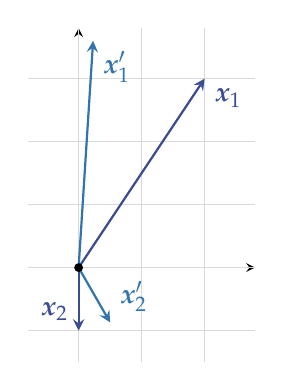
\begin{tikzpicture}[
                      scale=0.8,
                      >=stealth,
                  ]
                  \tikzset{
                      vec_p/.style = {thick, cyan!20!blue!80!black},
                      vec_i/.style = {thick, cyan!60!blue!80!black},
                  }

                  % Axes
                  \draw[->] (-0.8,0) -- (2.8,0);
                  \draw[->] (0,-1.5) -- (0,3.8);

                  % Grid
                  \draw[help lines, gray!30] (-0.8,-1.5) grid (2.8,3.8);

                  % New vectors x1', x2'
                  \draw[->, vec_i] (0,0) -- (0.23,3.60) node[below right] {$\vect{x}'_1$};
                  \draw[->, vec_i] (0,0) -- (0.5,-0.87) node[above right] {$\vect{x}'_2$};

                  % Original vectors x1, x2
                  \draw[->, vec_p] (0,0) -- (2,3) node[below right] {$\vect{x}_1$};
                  \draw[->, vec_p] (0,0) -- (0,-1) node[above left] {$\vect{x}_2$};

                  % Origin
                  \fill (0,0) circle (2pt);

              \end{tikzpicture}
          }

\end{enumerate}

\end{document}
